\documentclass[%
	11pt,
	a4paper,
	utf8,
	%twocolumn
		]{article}	

\usepackage{style_packages/podvoyskiy_article_extended}


\begin{document}
\title{Заметки по машинному обучению и анализу данных}

\author{\itshape Подвойский А.О.}

\date{}
\maketitle

\thispagestyle{fancy}

Здесь приводятся заметки по некоторым вопросам, касающимся машинного обучения, анализа данных, программирования на языках \texttt{Python}, \texttt{R} и прочим сопряженным вопросам так или иначе, затрагивающим работу с данными.


\shorttableofcontents{Краткое содержание}{1}


\tableofcontents

\section{Основные термины}

\noindent\emph{Квантиль} -- значение, которое заданная случайная величина не превышает с фиксированной вероятностью. Если вероятность задана в процентах, то квантиль называют процентилем. Пример: фраза <<90-й процентиль массы тела у новорожденных мальчиков составляет 4 кг>>, что означает 90\% мальчиков рождаются с массой тела, меньшей или в частном случае равной 4 кг, а 10\% соответственно -- с массой большей 4 кг. Если распределение непрерывно, то $ \alpha $-квантиль однозначно задается уравнением
\begin{align*}
	F_X(x_\alpha) = \alpha.
\end{align*}

Для непрерывных распределений справедливо следующее широко использующееся при построении доверительных интервалов равенство
\begin{align*}
	\mathbb{P}\big(x_{\frac{1 - \alpha}{2}} \leqslant X \leqslant x_{\frac{1 + \alpha}{2}}\big) = \alpha.
\end{align*}

\noindent\emph{Интерквартильный размах} -- разность между третьим и первым квартилями, то есть $ x_{0,75} - x_{0,25} $. Интерквартильный размах является характеристикой разброса и является робастным аналогом дисперсии. Вместе, медиана и интерквартильный размах могут быть использованы вместо математического ожидания и дисперсии в случае распределений с большими выбросами.

\section{Теория алгоритмов и структуры данных}

В \emph{теории сложности вычислений} широкое распространение получило обозначение <<\emph{О}-большое>>. Типичный результат выглядит следующим образом: <<данный алгоритм работает за время $ O(n^2 \log n) $>>, и его следует понимать как <<существует такая константа $ C > 0 $, что \emph{время работы} алгоритма в \emph{наихудшем} случае не превышает $ C\,n^2 \log n $, начиная с некоторого $ n $>>.

Практическая ценность асимптотических результатов такого рода зависит от того, насколько мала неявно подразумеваемая константа $ c $. Как мы уже отмечали выше, для подавляющего большинства известных алгоритмов она находится в разумных пределах, поэтому, как правило, имеет место следующий тезис: алгоритмы, более эффективные с точки зрения их асимптотического поведения, оказываются также более эффективными и при тех сравнительно небольших размерах входных данных, для которых они реально используются на практике. Другими словами, \emph{асимптотические оценки эффективности} достаточно полно отражают реальное положение вещей.

Теория сложности вычислений по определению считает, что алгоритм, работающий за время $ O(n^2 \log n) $ лучше алгоритма с временем работы $ O(n^3) $, и в подавляющем большинстве случаев это отражает реально существующую на практике ситуацию.


\section{Градиентный бустинг}

\subsection{Общие сведения}

\subsection{Особенности реализации в пакете \texttt{sklearn}}

\subsection{Особенности реализации в пакете \texttt{XGBoost}}

\subsubsection{Установка пакета \texttt{xgboost} на \texttt{Windows}}

Устанавливать пакет \texttt{xgboost} рекомендуется с помощью следующей команды

\begin{lstlisting}[
numbers = none
]
conda install -c anaconda py-xgboost 
\end{lstlisting}

Существует альтернативный способ установки пакета \texttt{xgboost} (разумеется он работает и для других пакетов). Для начала требуется вывести список доступных каналов (см. \pic{fig:xgboost_conda_search}), по которым будет проводиться поиск интересующего пакета (в данном случае пакета \texttt{xgboost}), а затем можно воспользоваться конструкцией

\begin{lstlisting}[
numbers = none
]
anaconda search -t conda xgboost
\end{lstlisting}

\begin{figure}[h]
	\centering
	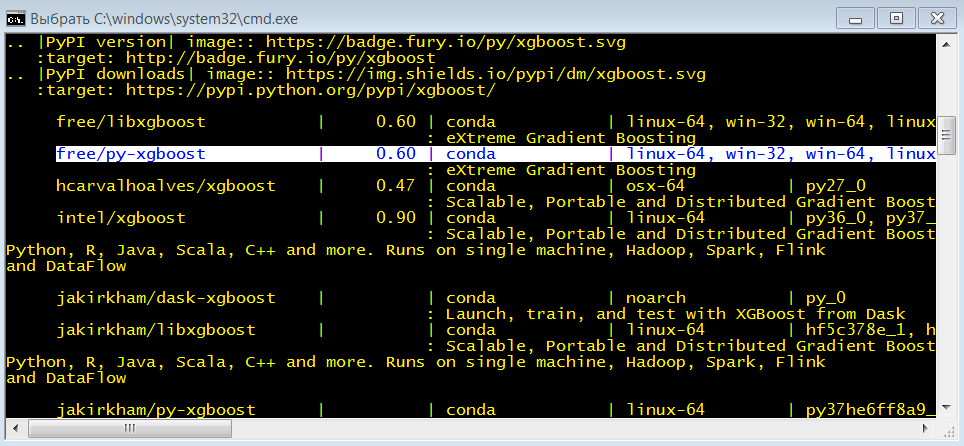
\includegraphics[scale=0.85]{figures/xgboost_conda_search.png}
	\caption{Окно командной оболочки \texttt{cmd.exe} со списком доступных каналов, по которым будет проводиться поиск пакета \texttt{xgboost} }\label{fig:xgboost_conda_search}
\end{figure}


После, выбрав канал, можно приступать к установке пакета

\begin{lstlisting}[
numbers = none
]
conda install -c free py-xgboost
\end{lstlisting}

\subsubsection{Простой пример работы с \texttt{xgboost} и \texttt{shap}}

Решается задача бинарной классификации. Требуется построить модель, предсказывающую годовой доход заявителя по порогу \$50'000 (то есть больше или меньше \$50'000 зарабатывает заявитель в год). Используется набор данных  UCI Adult income

\begin{lstlisting}[
style = ironpython,
numbers = none
]
import xgboost
import shap  # для оценки важности признаков вычисляются значения Шепли (Shapley value)
import numpy as np
import matplotlib.pyplot as plt
from sklearn.model_selection import train_test_split

shap.initjs()

X, y = shap.datasets.adult()
X_display, y_display = shap.datasets.adult(display=True)

X_train, X_test, y_train, y_test = train_test_split(X, y, test_size=0.2, random_state=7)
d_train = xgboost.DMatrix(X_train, label=y_train)
d_test = xgboost.DMatrix(X_test, label=y_test)

params = {
    'eta' : 0.01,
    'objective' : 'binary:logistic',
    'subsample' : 0.5,
    'base_score' : np.mean(y_train),
    'eval_metric' : 'logloss'        
}
model = xgboost.train(params, d_train,
                      num_boost_round = 5000,  # число итераций бустинга
                      evals = [(d_test, 'test')],
                      verbose_eval=100,  # выводит результат на каждой 100-ой итерации бустинга
                      early_stopping_rounds=20)

xgboost.plot_importance(model)
\end{lstlisting}

На \pic{fig:xgboost_plot}, \pic{fig:xgboost_plot_cover} и \pic{fig:xgboost_plot_gain} изображены графики важности признаков.

\begin{figure}[h]
	\centering
	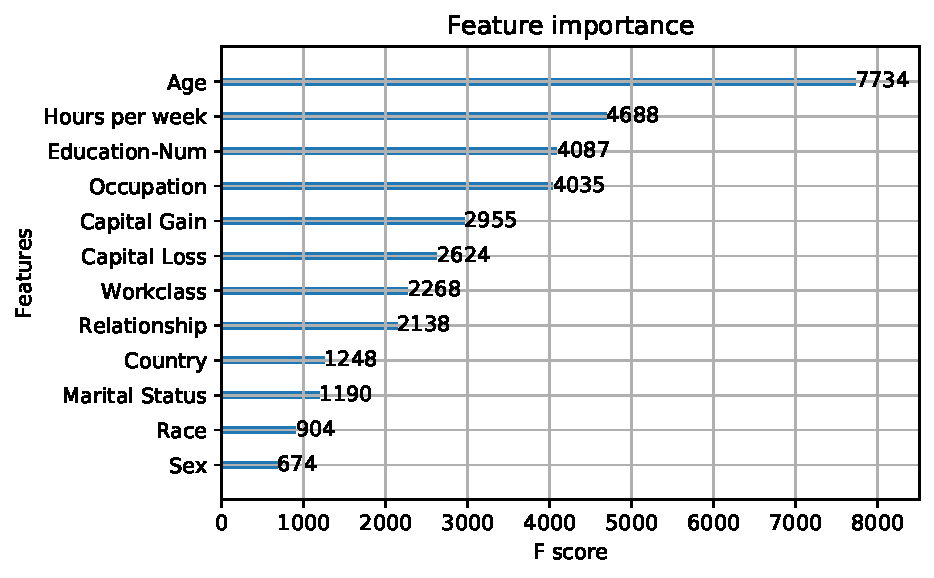
\includegraphics[scale=0.75]{figures/xgboost.plot.pdf}
	\caption{График важности признаков \lstinline{xgboost.plot_importance(model)},\\построенный с помощью пакета \texttt{xgboost} }\label{fig:xgboost_plot}
\end{figure}

\begin{figure}[h]
	\centering
	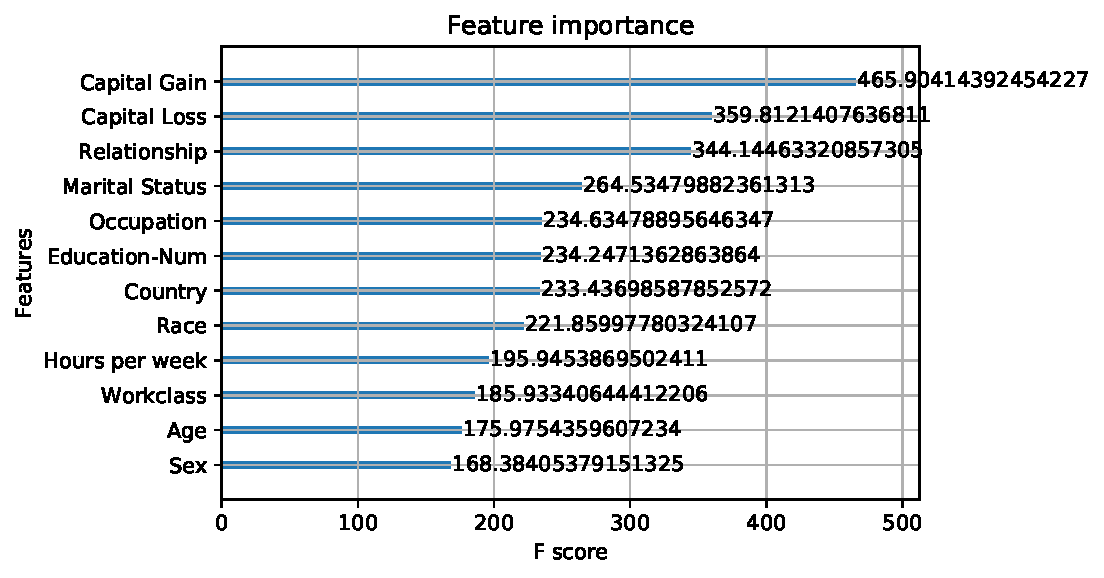
\includegraphics[scale=0.75]{figures/xgboost.plot.cover.pdf}
	\caption{График важности признаков \lstinline{xgboost.plot_importance(model, importance_type='cover')},\\построенный с помощью пакета \texttt{xgboost} }\label{fig:xgboost_plot_cover}
\end{figure}

\begin{figure}[h]
	\centering
	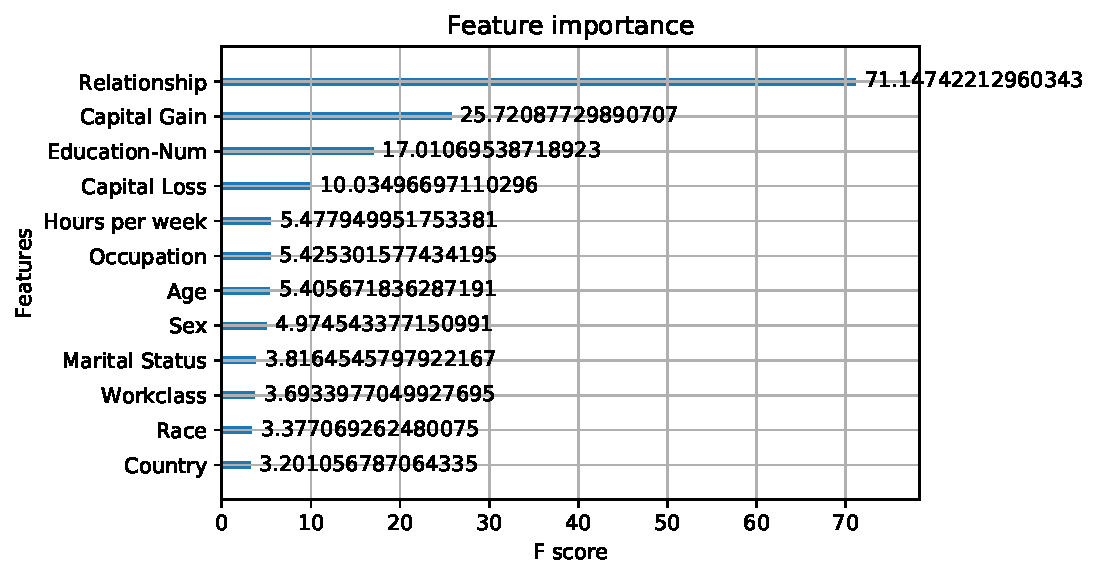
\includegraphics[scale=0.75]{figures/xgboost.plot.gain.pdf}
	\caption{График важности признаков \lstinline{xgboost.plot_importance(model, importance_type='gain')},\\построенный с помощью пакета \texttt{xgboost} }\label{fig:xgboost_plot_gain}
\end{figure}

Следует иметь в виду, что в библиотеке \texttt{xgboost} поддерживается три варианта вычисления важности признаков (см.~\href{https://towardsdatascience.com/interpretable-machine-learning-with-xgboost-9ec80d148d27}{Interpretable Machine Learning with XGBoost}):

\begin{itemize}
	\item \texttt{weight}: общее число сценариев по всем деревьям, когда $i$-ый признак используется для расщепления обучающего набора данных,
	
	\item \texttt{cover}: общее число сценариев по всем деревьям, когда $i$-ый признак используется для расщепления набора данных, взвешенное по числу точек обучающего набора данных, которые проходят через эти расщепления,
	
	\item \texttt{gain}: среднее снижение потерь на обучающем наборе данных, полученное при использовании $i$-ого признака.
\end{itemize}


\subsection{Особенности реализации в пакете \texttt{LightGBM}}

\subsection{Особенности реализации в пакете \texttt{CatBoost}}

\section{Форматирование строк в языке \texttt{Python}}

Пример форматирования строк в \texttt{Python} 

\begin{lstlisting}[
style = ironpython,
numbers = none
]
'{:*>+12.3f}, {:#^+17.5G}, {!r}'.format(
                                     math.pi,
                                     -math.exp(1)*10**(+6),
                                     type(list)  # для этого объекта будет
                                                 # использована функция repr()
                                 )
# "******+3.142, ###-2.7183E+06###, <class 'type'>"
\end{lstlisting}

Часть, стоящая после двоеточия, называется \emph{спецификатором формата} \cite[\strbook{283}]{ramalho:python-2016}. Полезные приемы форматирования можно найти в \cite{prohorenok:python-2016}.

\section{Хэшируемые пользовательские классы в языке \texttt{Python}}

Чтобы класс был хэшируемым\footnote{Обычно говорят, что объект называется хэшируемым если i) у него есть хэш-значение, которое не изменяется пока объект существует, и ii) объект поддерживает сравнение с другими объектами. Однако на мой взгляд лучше сказать, что объект является хэшируемым, если его структура не может изменяется и он поддерживает сравнение с другими объектами}, следует реализовать метод \texttt{\_\_hash\_\_}. Нужно также, чтобы векторы были \emph{неизменяемыми}. И этого можно добиться, сделав компоненты \texttt{x} и \texttt{y} свойствами, доступными только для чтения.

\begin{lstlisting}[
title = {\sffamily Пример неизменяемого, но нехэшируемого класса},
style = ironpython,
emph = {__init__, x, y, __iter__, __repr__, __str__, angle, __format__,
__bytes__, __eq__, __abs__, __bool__},
numbers = none
]
import array
import math

class Vector2d:
    '''
    Неизменяемый, но еще нехэшируемый класс
    '''
    typecode = 'd'

    def __init__(self, x, y):
        self.__x = x  # закрытый атрибут экземпляра класса
        self.__y = y  # закрытый атрибут экземпляра класса

    # открытое свойство; прочитать значение `x` можно, но нельзя передать новое значение
    @property  
    def x(self):
        return self.__x

    # открытое свойство; прочитать значение `y` можно, но нельзя передать новое значение
    @property  
    def y(self):
        return self.__y

    def __iter__(self):
        return (i for i in (self.x, self.y))

    def __repr__(self):
        class_name = type(self).__name__
        return '{}({!r}, {!r})'.format(class_name, *self)

    def __str__(self):
        return str(tuple(self))

    def angle(self):
        return math.atan2(self.y, self.x)

    def __format__(self, fmt_spec = ''):  # пользовательский формат
        if fmt_spec.endswith('p'):  # если спецификатор формата заканчивается на 'p',
                                    # то координаты выводятся в полярном формате
            fmt_spec = fmt_spec[:-1]
            coords = (abs(self), self.angle())
            outer_fmt = '<{}, {}>'
        else:
            coords = self
            outer_fmt = '({}, {})'
        components = (format(c, fmt_spec) for c in coords)
        return outer_fmt.format(*components)

    def __bytes__(self):
        return (bytes([ord(self.typecode)]) + bytes(array(self.typecode, self)))

    def __eq__(self, other):
        return tuple(self) == tuple(other)

    def __abs__(self):
        return math.hypot(self.x, self.y)

    def __bool__(self):
        return bool(abs(self))
\end{lstlisting}

То есть здесь декоратор \texttt{@property} помечает метод чтения свойств, который возвращает значение закрытого атрибута экземпляра класса \texttt{self.\_\_x} или \texttt{self.\_\_y}.

Так как в реализации класса есть метод \texttt{\_\_format\_\_}, можно печатать класс управляя форматом, например,

\begin{lstlisting}[
title = {\sffamily Пример использования класса с реализованным методом \texttt{\_\_format\_\_}},
style = ironpython,
numbers = none
]
>>> v1 = Vector2d(10, 5)
>>> '{:*^+12.3gp}'.format(v1)  # '<***+11.2****, ***+0.464***>'
>>> '{:.3f}'.format(v1)  # '(10.000, 5.000)'
\end{lstlisting}

Наконец, можно реализовать метод \texttt{\_\_hash\_\_}. Он должен возвращать \texttt{int} и в идеале учитывать хэши объектов-атрибутов, потому что у равных объектов хэши также должны быть одинаковыми.

В документации по специальному методу \texttt{\_\_hash\_\_} рекомендуется объединять хэши компонентов с помощью побитового оператора\footnote{Побитовые операторы рассматривают операнды как бинарные последовательности} \emph{исключающего ИЛИ} (\texttt{\^}) \cite[\strbook{287}]{ramalho:python-2016}

\begin{lstlisting}[
style = ironpython,
emph = {__hash__},
numbers = none
]
...
def __hash__(self):
    return hash(self.__x) ^ hash(self.__y)  # побитовое исключающее ИЛИ
\end{lstlisting}

Теперь класс \texttt{Vector2d} стал \emph{хэшируемым}.

\begin{lstlisting}[
style = ironpython,
numbers = none
]
>>> v1 = Vector2d(3, 4)
>>> v2 = Vector2d(3.1, 4.2)
>>> hash(v1), hash(v2)  # (7, 384307168202284039)
>>> set([v1, v2])  # {Vector2d(3, 4), Vector2d(3.1, 4.2)}
\end{lstlisting}

\remark{
Строго говоря, для создания хэшируемого типа необязательно вводить свойства или как-то иначе защищать атрибуты экземпляра класса от изменения. Требуется только корректно реализовать методы \texttt{\_\_hash\_\_} и \texttt{\_\_eq\_\_}. Но хэш-значения экземпляра никогда не должно изменяться \cite[\strbook{288}]{ramalho:python-2016}
}

\section{Как интерпретировать связь между именем функции и объектом функции в \texttt{Python}}

Рассмотрим класс, который печатает выводимые в терминал строки в обратном порядке

\begin{lstlisting}[
style = ironpython,
emph = {LookingGlass, __enter__, reverse_write, __exit__},
]
class LookingGlass:
    def __enter__(self):
        import sys
        # атрибут экземпляра класса self.original_write -> объект функции sys.stdout.write
        self.original_write = sys.stdout.write  
        # переменная sys.stdout.write -> объект функции self.reverse_write
        sys.stdout.write = self.reverse_write  
        return 'jabberwocky'.upper()
        
    def reverse_write(self, text):
        self.original_write(text[::-1])
        
        
    def __exit__(self, exc_type, exc_value, traceback):
        import sys
        # переменная sys.stdout.write "через" атрибут экземпляра self.original_write 
        # ссылается на объект функции sys.stdout.write
        sys.stdout.write = self.original_write
\end{lstlisting}

В методе \texttt{\_\_enter\_\_} есть несколько неочевидных нюансов. В строке 4 атрибут экземпляра класса \texttt{self.original\_write} получает ссылку на метод \texttt{write} стандартного потока вывода, а в строке 5 <<как бы метод>> \texttt{sys.stdout.write} получает ссылку на метод экземпляра класса \texttt{self.reverse\_write} и кажется, что должен был бы образоваться рекурсивный вызов, но на самом деле это не так. Дело в том, что значение имеет с какой стороны от оператора \texttt{=} стоит имя функции: если слева, то это \emph{имя переменной}, а если справа, то это \emph{объект функции}.

Итак, по порядку: в строке 4 атрибут экземпляра класса \texttt{self.original\_write} получает ссылку на \emph{объект функции} \texttt{sys.stdout.write}, а в 5-ой строке \emph{переменная} \texttt{sys.stdout.write} получает ссылку на \emph{объект функции} (метод экземпляра класса) \texttt{self.reverse\_write}, который <<через>> атрибут экземпляра \texttt{self.original\_write} вызывает \emph{объект функции} \texttt{sys.stdout.write}.

А в строке 18, мы возвращаем все как было, т.е. \emph{переменная} \texttt{sys.stdout.write} получает ссылку на \emph{объект функции} \texttt{sys.stdout.write}.

Рассмотрим более простой пример (см. \pic{fig:variable_with_link_function})

\begin{lstlisting}[
style = ironpython,
numbers = none
]
>>> def f(): pass  # переменная f -> объект функции f()
>>> def g(): pass  # переменная g -> объект функции g()
# модель: переменная -> объект
>>> a = f  # переменная a -> объект функции f()
>>> f = g  # переменная f -> объект фукнции g()
# НИКАКОЙ ТРАНЗИТИВНОСТИ!
>>> a  # <function __main__.f()>
>>> f  # <function __main__.g()>
\end{lstlisting}

То есть, когда объявляется функция, например, \texttt{def f(): pass}, то создается \emph{переменная} \texttt{f}, которая получает ссылку на \emph{объект функции} \texttt{f()}.

\remark{
Даже если используется одно и тоже имя \texttt{f}: слева от оператора присваивания \texttt{f} -- это \emph{переменная}, а справа от оператора \texttt{f} -- это \emph{объект} (например, объект функции), так как в \texttt{Python} переменные ссылаются только на объекты!
}

\begin{figure}[h]
	\centering
	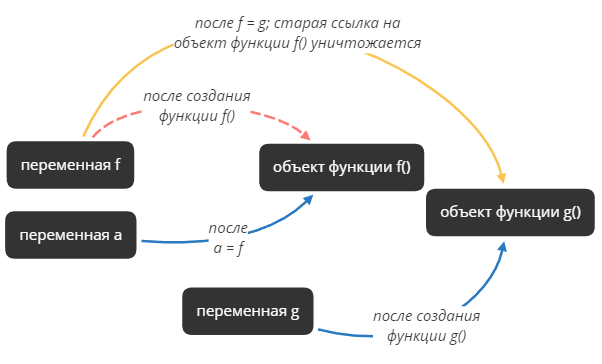
\includegraphics[scale=0.85]{figures/variable_with_link_function.png}
	\caption{ Схема, описывающая связи между именами функций и их объектами }\label{fig:variable_with_link_function}
\end{figure}

\section{Использование \texttt{@contextmanager}}

Если \emph{генератор} снабжен декоратором \texttt{@contextmanager}, то \texttt{yield} разбивает тело функции на две части:

\begin{itemize}
	\item все, что находится до \texttt{yield}, исполняется в начале блока \texttt{with}, когда интерпретатор вызывает метод \texttt{\_\_enter\_\_} ,
	
	\item а все, что находится после \texttt{yield}, выполняется при вызове метода \texttt{\_\_exit\_\_} в конце блока.
\end{itemize}

Например,

\begin{lstlisting}[
style = ironpython,
title = {\sffamily неудачный пример},
emph = {looking_glass, reverse_write}
]
# mirror_gen.py
import contextlib

@contextlib.contextmanager  # декорируем генераторную функцию
def looking_glass():  # генераторная функция
    import sys
    original_write = sys.stdout.write  # (1)
    
    def reverse_write(text):  # замыкание
        original_write(text[::-1])  # здесь original_write -- свободная переменная
    
    sys.stdout.write = reverse_write  # (2)
    # все что выше `yield` выполняется в начале блока with
    yield 'jabberwocky'.upper()  # (3)
    # все что ниже `yield` выполняется в конце блока with
    sys.stdout.write = original_write  # (4)
\end{lstlisting}

Комментарии к коду:

\begin{itemize}
	\item (1) -- локальная \emph{переменная} \texttt{original\_write} получает ссылку на \emph{объект функции} (вернее на объект метода) стандартного потока вывода; теперь вызывая \texttt{original\_write} мы будет вызывать \texttt{sys.stdout.write},
	
	\item (2) -- переменная \texttt{write} из подмодуля \texttt{stdout} модуля \texttt{sys} получает ссылку на \emph{замыкание} \texttt{reverse\_write} (функцию с расширенной областью видимости, которая включает все неглобальные переменные); теперь, когда мы вызываем \texttt{sys.stdout.write} будет вызываться \\ \texttt{reverse\_write}, который в свою очередь будет вызывать \texttt{original\_write}, вызывающий метод \texttt{sys.stdout.write} и передавать ему обращенную строку,
	
	\item (3) -- здесь функция приостанавливается на время выполнения блока \texttt{with},
	
	\item (4) -- когда поток выполнения покидает блок \texttt{with} любым способом, выполнение функции возобновляется с места, следующего за \texttt{yield}; в данном случае восстанавливается исходный метод \texttt{sys.stdout.write}
\end{itemize}

Пример работы функции

\begin{lstlisting}[
style = ironpython,
numbers = none
]
>>> from mirror_gen import looking_glass

>>> with looking_glass() as what:
        print('Alice, Kitty and Snowdrop')  # pordwonS dna yttiK ,ecilA
        print(what)                         # YKCOWREBBAJ
\end{lstlisting}

По существу декоратор \texttt{@contextlib.contextmanager} обертывает функцию классом, который реализует методы \texttt{\_\_enter\_\_} и \texttt{\_\_exit\_\_}\footnote{Этот класс называется \texttt{\_GeneratorContextManager}}.

Метод \texttt{\_\_enter\_\_} этого класса выполняет следующие действия \cite[\strbook{488}]{ramalho:python-2016}:

\begin{enumerate}
	\item Вызывает \emph{генераторную функцию} \texttt{looking\_glass()}\footnote{При вызове генераторной функции возвращается объект-генератор} и запоминает объект-генератор (пусть называется \texttt{gen}),
	
	\item Вызывает \texttt{next(gen)}, чтобы заставить генератор выполнить код до предложения \texttt{yield},
	
	\item Возвращает значение, отданное \texttt{next(gen)}, чтобы его можно было связать с переменной в части \texttt{as} блока \texttt{with}, т.е. строка, отданная инструкцией \texttt{yield} связывается с переменной \texttt{what}.
\end{enumerate}

По завершении блока \texttt{with} метод \texttt{\_\_next\_\_} выполняет следующие действия:

\begin{enumerate}
	\item Смотрит, было ли передано исключение в параметре \texttt{exc\_type}; если да, вызывает \\ \texttt{gen.throw(exception)}, в результате чего строка в теле генераторной функции, содержащая \texttt{yield}, возбуждает исключение,
	
	\item В противном случае вызывает \texttt{next(gen)}, что приводит к выполнению части генераторной функции после \texttt{yield}.
\end{enumerate}

В рассмотренном примере есть очень серьезный дефект: если в теле блока \texttt{with} возникает исключение, то интерпретатор перехватывает его и повторно возбуждает в выражении \texttt{yield} внутри \texttt{looking\_glass}. Но здесь нет никакой обработки исключений, поэтому функция аварийно завершается, оставив систему в некорректном состоянии.

Более аккуратный вариант генераторной функции приведен ниже

\begin{lstlisting}[
title = {\sffamily Правильный вариант},
emph = {looking_glass, reverse_write},
style = ironpython,
numbers = none
]
# mirror_gen_exc.py
import contextlib

@contextlib.contextmanager
def looking_glass():  # здесь генераторная функция работает скорее как сопрограмма
    import sys
    original_write = sys.stdout.write  # переменная получает -> на объект функции write

    def reverse_write(text):  # замыкание
        original_write(text[::-1])

    sys.stdout.write = reverse_write  # переменная write получает -> на замыкание reverse_write
    msg = ''
    try:
        yield 'jabberwocky'.upper()  # отдает строку и переключается на блок with
    except ZeroDivisionError:
        msg = 'Пожалуйста не делите на ноль!'
    finally:  # выполняется в любом случае
        sys.stdout.write = original_write  # переменная write получает -> на объект функции write
        if msg:  # if msg != ''
            print(msg)
\end{lstlisting}

Пример выполнения

\begin{lstlisting}[
style = ironpython,
numbers = none
]
>>> from mirror_gen_exc import looking_glass
>>> with looking_glass() as what:
        print('aaaabb')  # bbaaaa
        print(5/0)       # Пожалуйста не делите на ноль!
\end{lstlisting}

\remark{
Отметим, что использование слова \texttt{yield} в генераторе, который используется совместно с декоратором \texttt{@contextmanager}, не имеет ничего общего с итерированием. В рассмотренных примерах генераторная функция работает скорее, как \emph{сопрограмма}: процедура, которая доходит до определенной точки, затем приостанавливается и дает возможность поработать клиентскому коду до тех пор, пока он не захочет возобновить выполнение процедуры с прерванного места
}

\section{Перегрузка операторов в языке \texttt{Python}}

Перегрузка операторов позволяет экземплярам классов участвовать в обычных операциях \cite{prohorenok:python-2016}.

Основы перегрузки операторов:

\begin{itemize}
	\item запрещается перегружать операторы для встроенных типов,
	
	\item запрещается создавать новые операторы, можно перегружать существующие,
	
	\item несколько операторов нельзя перегружать вовсе: \texttt{is}, \texttt{and}, \texttt{or}, \texttt{not} (на побитовые операторы это не распространяется)
\end{itemize}

Фундаментальное правило: инфиксный оператор всегда возвращает \emph{новый объект}, т.е. создает новый экземпляр (составные операторы изменяемых объектов возвращают \texttt{self}, т.е. изменяют левый операнд на месте).

Иначе говоря, в случае инфиксных операторов нельзя модифицировать \texttt{self}, а нужно создавать и возвращать новый экземпляр подходящего типа \cite[\strbook{405}]{ramalho:python-2016}.

\remark{
\emph{Инфиксные} операторы (\texttt{*}, \texttt{+} и т.д.) независимо от типа данных всегда возвращают \emph{новый объект}. \emph{Составные} операторы (\texttt{+=}, \texttt{*=} и пр.) для объектов \emph{неизменяемого} типа данных (кортежи, строки и пр.) возвращают новый объект, но в случае объектов \emph{изменяемого} типа данных (списки) -- изменяют объект на месте
}

\begin{lstlisting}[
style = ironpython,
title = {\sffamily Сравнение работы инфиксных и составных операторов},
numbers = none
]
# изменяемый объект
>>> lst = [100]  
>>> id(lst)  # 179426376
>>> lst = lst*2  # инфиксный оператор возвращает новый объект, поэтому id будет другим
>>> id(lst)  # 117159368 -- изменился
>>> lst  # [100, 100]
>>> lst *= 2  # но составной оператор для изменяемого объекта изменяет левый операнд на месте
>>> lst  # [100, 100, 100, 100]
>>> id(lst)  # 117159368 -- не изменился
# неизменяемый объект
>>> tpl = (100,)
>>> id(tpl)  # 114189896
>>> tpl = tpl*2  # инфиксный оператор вернет новый объект
>>> tpl  # (100, 100)
>>> id(tpl)  # 82350344 -- изменился
>>> tpl *= 2  # составной оператор создаст новый объект и перепривяжет его к tpl
>>> tpl # (100, 100, 100, 100)
>>> id(tpl)  # 93229768 -- изменился
\end{lstlisting}

При умножении \emph{последовательности} (списки, кортежи, строки) на \emph{целое число} создается копия последовательности заданное число раз, а затем копии склеиваются. 

Как читать выражения с математическими операторами:
\begin{itemize}
	\item Смотрим к какому классу относится оператор: \emph{инфиксному} или \emph{составному},
	
	\item Если оператор инфиксный, то независимо от того являются операнды изменяемыми или нет будет возвращен новый объект\footnote{При условии, что оператор в случае данных операндов имеет смысл},
	
	\item Если оператор составной, то нужно выяснить является левый операнд изменяемым или нет,
	\begin{itemize}
		\item левый операнд изменяемый: составной оператор изменит левый операнд на месте (идентификатор не изменится),
		
		\item левый операнд неизменяемый: составной оператор создаст новый объект и перепривяжет его к переменной (изменится идентификатор).
	\end{itemize}
\end{itemize}

\subsection{Перегрузка оператора сложения}

Для поддержки операций с объектами \emph{разных типов} в \texttt{Python} имеется особый механизм диспетчеризации для специальных методов, ассоциированных с инфиксными операторами.

Видя выражение \texttt{a + b}, интерпретатор выполняет следующие шаги:

\begin{itemize}
	\item Если у \texttt{a} есть метод \texttt{\_\_add\_\_}, вызвать \texttt{a.\_\_add\_\_(b)} и вернуть результат, если только он не равен \texttt{NotImplemented}\footnote{\texttt{NotImplemented} -- это значение-синглтон, которое должен возвращать специальный метод инфиксного оператора, чтобы сообщить интерпретатору, что не умеет обрабатывать данный операнд} (т.е. оператор не знает как обрабатывать данный операнд),
	
	\item Если у левого операнда \texttt{a} нет метода \texttt{\_\_add\_\_} или его вызов вернул \texttt{NotImplemented}, проверить, есть ли у правого операнда \texttt{b} <<правый>> метод \texttt{\_\_radd\_\_}\footnote{Иногда такие методы называют <<инверсными>> методами, но лучше их представлять как \emph{правые} методы, так как они вызываются от имени правого операнда}, и, если да, вызвать \texttt{b.\_\_radd\_\_(a)} и вернуть результат, если только он не равен \texttt{NotImplemented},
	
	\item Если у \texttt{b} нет метода \texttt{\_\_radd\_\_} или его вызов вернул \texttt{NotImplemented}, возбудить исключение \texttt{TypeError}.
\end{itemize}

Рассмотрим реализацию методов сложения для объектов

\begin{lstlisting}[
style = ironpython,
emph = {VectorUser, __add__, __radd__, __iter__, __init__, __repr__},
numbers = none
]
import itertools
import reprlib

class VectorUser:
    def __init__(self, seq):
        self._seq = array('d', seq)

    def __iter__(self):
        return iter(self._seq)

    def __repr__(self):
        components = reprlib.repr(self._seq)
        components = components[components.find('['):-1]
        return f'Vector({components})'

    def __add__(self, other):
        try:
            pairs = itertools.zip_longest(self, other, fillvalue=0.0)
            return VectorUser(a + b for a, b in pairs)  # возвращает новый экземпляр класса
        except TypeError:
            return NotImplemented

    def __radd__(self, other):
        return self + other
\end{lstlisting}

Как работает этот код. Рассмотрим случай, когда экземпляр класса \texttt{Vector} находится слева от оператора \texttt{+}

\begin{lstlisting}[
style = ironpython,
numbers = none
]
>>> v1 = VectorUser([3, 4, 5])
>>> v1 + (10, 20, 30)  # Vector([13.0, 24.0, 35.0])
# v1.__add__((10, 20, 30))
# удобно представлять VectorUser.__add__(v1, (10, 20, 30))
\end{lstlisting}

Первым делом интерпретатор пытается выяснить есть ли у левого операнда метод \texttt{\_\_add\_\_}. В данном случае у объекта \texttt{v1} есть такой метод, поэтому ничто не мешает вызвать его напрямую. Аргумент \texttt{self} метода \texttt{\_\_add\_\_} получает ссылку на \texttt{v1} (экземпляр класса \texttt{Vector}), а \texttt{other} -- ссылку на кортеж. Далее с помощью \texttt{zip\_longest} конструируется генератор кортежей, который в следующей строке используется в генераторном выражении при создании нового экземпляра класса \texttt{Vector} (оператор должен возвращать новый объект).

Теперь рассмотрим случай, когда экземпляр класса \texttt{VectorUser} находится справа от оператора \texttt{+}

\begin{lstlisting}[
style = ironpython,
numbers = none
]
>>> (10, 20, 30) + v1
\end{lstlisting}

И снова интерпретатор пытается выяснить есть ли у левого операнда метод \texttt{\_\_add\_\_}. У кортежа есть такой метод, но он не умеет работать с объектом \texttt{VectorUser} (возвращает \texttt{NotImplemented}).

Теперь интерпретатор проверяет есть ли у правого операнда <<правый>> метод \texttt{\_\_radd\_\_}. Правый операнд это экземпляр класса \texttt{VectorUser}, поэтому \texttt{v1.\_\_radd\_\_((10, 20, 30))} это то же самое что и \texttt{VectorUser.\_\_radd\_\_(v1, (10, 20, 30))}.

Другими словами, аргумент \texttt{self} метода \texttt{\_\_radd\_\_} получает ссылку на объект \texttt{v1}, а аргумент \texttt{other} -- ссылку на кортеж. И тогда в выражении \texttt{self + other}, которое возвращается методом \texttt{\_\_radd\_\_}, экземпляр класса \texttt{VectorUser} окажется слева от оператора \texttt{+}. Интерпретатор, встретив выражение \texttt{self + other}, начинает с поиска метода \texttt{\_\_add\_\_} у левого операнда и, найдя его, возвращает новый экземпляр класса \texttt{VectorUser(...)}.

\remark{
Еще раз: чтобы поддержать операции с \emph{разными типами}, мы возвращаем специальное значение \texttt{NotImplemented} -- не исключение, -- давая интерпретатору возможность попробовать еще раз: поменять операнды местами и вызывать специальный инверсный (правый) метод, соответствующий тому же оператору (например, \texttt{\_\_radd\_\_})
}

\subsection{Перегрузка оператора умножения на скаляр}

Рассмотрим в качестве примера умножение вектора \texttt{VectorUser} на скаляр

\begin{lstlisting}[
style = ironpython,
emph = {__mul__, __rmul__},
numbers = none
]
import numbers

# внутри класса VectorUser
def __mul__(self, scalar):
    if isinstance(scalar, numbers.Real):  # сравнение с абстрактным базовым классом
        return VectorUser(n*scalar for n in self)
    else:
        return NotImplemented

def __rmul__(self, scalar):
    return self*scalar
\end{lstlisting}

\begin{lstlisting}[
style = ironpython,
numbers = none
]
>>> v1 = VectorUser([3, 4, 5])
>>> v1*4  # Vector([12.0, 16.0, 20.0])
>>> 10*v1 # Vector([30.0, 40.0, 50.0])
\end{lstlisting}

В первом случае интерпретатор начинает с поиска метода \texttt{\_\_mul\_\_} у левого операнда. Метод найден, объект справа (число 4) действительно является экземпляром подкласса абстрактного базового класса \texttt{numbers.Real}. Значит теперь можно вернуть экземпляр \texttt{VectorUser}.

Во втором случае интерпретатор так же начинает с поиска метода \texttt{\_\_mul\_\_} у левого операнда и не находит его. Поэтому на следующем шаге ищется правый метод \texttt{\_\_rmul\_\_} у правого операнда. Теперь объект \texttt{v1} в выражении \texttt{self*scalar} стоит слева и потому в методе \texttt{\_\_rmul\_\_} аргумент \texttt{self} ссылается на \texttt{v1}, а \texttt{scalar} -- на \texttt{4}. Видя выражение \texttt{self*scalar} интерпретатор вызывает метод \texttt{\_\_mul\_\_}, который на этот раз выполняется без проблем.



\remark{
В общем случае, если прямой инфиксный метод (например, \texttt{\_\_mul\_\_}) предназначен для работы только с операндами того же типа, что и \texttt{self}, бесполезно реализовывать соответствующий инверсный метод (например, \texttt{\_\_rmul\_\_}), потому что он, по определению, вызывается, только когда второй операнд имеет другой тип \cite[\strbook{425}]{ramalho:python-2016}
}

\subsection{Операторы сравнения}

Обработка операторов сравнения (\texttt{==}, \texttt{!=}, \texttt{>}, \texttt{<=} и т.д.) интерпретатором \texttt{Python} похожа на обработку инфиксных операторов, но есть два важных отличия \cite[\strbook{417}]{ramalho:python-2016}:

\begin{itemize}
	\item для прямых и инверсных (правых) методов служит один и тот же набор методов; например, в случае оператора \texttt{==} как прямой, так и правый вызов обращаются к методу \texttt{\_\_eq\_\_}, но изменяется порядок аргументов.
	
	\item в случае \texttt{==} и \texttt{!=}, если инверсный (правый) вызов завершается ошибкой, то \texttt{Python} сравнивает идентификаторы объектов, а не возбуждает исключение (см.~\tblref{tab:operators_comp}).
\end{itemize}

\begin{table}[h]
	\centering
	\caption{\itshape Операторы сравнения. Инверсные (правые) методы вызываются, когда\\ прямой вызов вернул \texttt{NotImplemented}}\label{tab:operators_comp}
	%\renewcommand{\arraystretch}{1.05}
	\begin{tabular}{lllll}
		{Группа} & {Инфиксный} & Прямой вызов & Инверсный вызов & Запасной вариант \\
		{} & оператор & метода & метода & {} \\ \hline\hline
		Равенство & \texttt{a == b} & \texttt{a.\_\_eq\_\_(b)} & \texttt{b.\_\_eq\_\_(a)} & \texttt{return id(a) == id(b)} \\
		\rowcolor[gray]{0.96} {} & \texttt{a != b} & \texttt{a.\_\_ne\_\_(b)} & \texttt{b.\_\_ne\_\_(a)} & \texttt{return not (a == b)} \\
		\hline
		Порядок & \texttt{a > b} & \texttt{a.\_\_gt\_\_(b)} & \texttt{a.\_\_lt\_\_(b)} & \texttt{raise TypeError} \\
		\rowcolor[gray]{0.96} {} & \texttt{a < b} & \texttt{a.\_\_lt\_\_(b)} & \texttt{a.\_\_gt\_\_(b)} & \texttt{raise TypeError} \\
		{} & \texttt{a >= b} & \texttt{a.\_\_ge\_\_(b)} & \texttt{a.\_\_le\_\_(b)} & \texttt{raise TypeError} \\
		\rowcolor[gray]{0.96} {} & \texttt{a <= b} & \texttt{a.\_\_le\_\_(b)} & \texttt{a.\_\_ge\_\_(b)} & \texttt{raise TypeError}
	\end{tabular}
\end{table}

Однако поведение оператора \texttt{==} пользовательских классов зависит от реализации метода \texttt{\_\_eq\_\_}. Например, пусть есть класс \texttt{Vector}

\begin{lstlisting}[
style = ironpython,
emph = {__eq__},
numbers = none
]
# в классе Vector
def __eq__(self, other):
    if isinstance(other, Vector):
        return (len(self) == len(other) and all(a == b for a, b in zip(self, other)))
    else:
        return NotImpemented
\end{lstlisting}

и какой-то другой класс \texttt{Vector2d}

\begin{lstlisting}[
style = ironpython,
emph = {__eq__},
numbers = none
]
# в классе Vector2d
def __eq__(self, other):
    retrun tuple(self) == tuple(other)
\end{lstlisting}

Если теперь сравнить экземпляры этих классов

\begin{lstlisting}[
style = ironpython,
numbers = none
]
>>> v1 = Vector([1, 2])
>>> v2 = Vector2d(1, 2)
>>> v1 == v2  # True
\end{lstlisting}
то порядок действий будет следующим:

\begin{itemize}
	\item для вычисления \texttt{v1 == v2} интерпретатор вызовет \texttt{Vector.\_\_eq\_\_(v1, v2)},
	
	\item метод \texttt{Vector.\_\_eq\_\_(v1, v2)} видет, что \texttt{v2} не является экземпляром класса \texttt{Vector} и возвращает \texttt{NotImplemented},
	
	\item получив значение \texttt{NotImplemented}, интерпретатор вызывает метод \texttt{\_\_eq\_\_} правого операнда, т.е. \texttt{v2}: \texttt{Vector2d.\_\_eq\_\_(v2, v1)},
	
	\item \texttt{Vector2d.\_\_eq\_\_(v2, v1)} преобразует оба операнда в кортежи и сравнивает их, результат оказывается равен \texttt{True}.
\end{itemize}

Теперь рассмотрим сравнение с кортежем

\begin{lstlisting}[
style = ironpython,
numbers = none
]
>>> t = (1, 2)
>>> v1 == t  # False
\end{lstlisting}

В этом случае:

\begin{itemize}
	\item для вычисления \texttt{v1 == t} \texttt{Python} вызывает \texttt{Vector.\_\_eq\_\_(v1, t)},
	
	\item метод \texttt{Vector.\_\_eq\_\_(v1, t)} видит, что кортеж \texttt{t} не является экземпляром класса \texttt{Vector} и возвращает \texttt{NotImplemented},
	
	\item получив результат \texttt{NotImplemented}, интерпретатор вызывает метод \texttt{\_\_eq\_\_} правого объекта, т.е. \texttt{tuple.\_\_eq\_\_(t, v1)}
	
	\item но \texttt{tuple.\_\_eq\_\_(t, v1)} ничего не знает о классе \texttt{Vector}, и поэтому возвращает \texttt{NotImplemented},
	
	\item если правый вызов вернул \texttt{NotImplemented}, то \texttt{Python} в качестве последнего средства сравнивает идентификаторы объектов, что в данном случае возвращает \texttt{False}
\end{itemize}




 
\section{Области видимости в языке \texttt{Python}}

Когда мы говорим о поиске значения имени применительно к программному коду, под термином \emph{область видимости} подразумевается \emph{пространство имен} -- то есть место в программном коде, где имени было присвоено значение \cite{lutz:learningpython-2011}.

В любом случае область видимости переменной (где она может использоваться) всегда определяется местом, где ей было присвоено значение.

\remark{%
Термины <<\emph{область видимости}>> и <<\emph{пространство имен}>> можно использовать как синонимичные
}

При каждом вызове функции создается новое \emph{локальное пространство имен}. Это пространство имен представляет локальное окружение, содержащее имена параметров функции, а также имена переменных, которым были присвоены значения в теле функции.

По умолчанию операция присваивания создает локальные имена (это поведение можно изменить с помощью \texttt{global} или \texttt{local}).

Схема разрешения имен в языке \texttt{Python} иногда называется \emph{правилом LEGB}\footnote{Local, Enclosing, Global, Built-in} \cite[\strbook{477}]{lutz:learningpython-2011}:

\begin{itemize}
	\item Когда внутри функции выполняется обращение к неизвестному имени, интерпретатор пытается отыскать его в четырех областях видимости -- в \emph{локальной}, затем в \emph{локальной области любой объемлющей функции} или в выражении \texttt{lambda}, затем в \emph{глобальной} и, наконец, во \emph{встроенной}. Поиск завершается, как только будет найдено первое подходящее имя.
	
	\item Когда внутри функции выполняется операция присваивания \lstinline{a=10} (а не обращения к имени внутри выражения), интерпретатор всегда создает или изменяет имя в \emph{локальной области видимости}, если в этой функции оно не было объявлено глобальным или нелокальным.
\end{itemize}

Пример

\begin{lstlisting}[
style = ironpython,
numbers = none
]
# глобальная область видимости
X = 99  

def func(Y):  # Y и Z локальные переменные
    # локальная область видимости
    Z = X + Y # X - глобальная переменная
    return Z
    
func(1)  # Y = 1
\end{lstlisting}

Переменные \texttt{Y} и \texttt{Z} являются \emph{локальными} (и существуют только во время выполнения функции), потому что присваивание значений обоим именам осуществляется внутри определения функции: присваивание переменной \texttt{Z} производится с помощью инструкции \texttt{=}, а \texttt{Y} -- потому что аргументы всегда передаются через операцию присваивания.

Когда внутри функции выполняется операция присваивания значения переменной, она всегда выполняется в \emph{локальном пространстве имен функции}

\begin{lstlisting}[
style = ironpython,
emph = {f},
numbers = none
]
a = 10  # глобальная область видимости

def f():
    a = 100  # локальная область видимости
    return a
\end{lstlisting}

В результате переменная \texttt{a} в теле функции ссылается на совершенно другой объект, содержащий значение 100, а не тот, на который ссылается внешняя переменная.

Переменные во вложенных функциях привязаны к \emph{лексической области видимости}. То есть поиск имени переменной начинается в \emph{локальной области видимости} и затем последовательно продолжается во всех \emph{объемлющих областях видимости внешних функций}, в направлении от внутренних к внешним.

Если и в этих \emph{пространствах имен} искомое имя не будет найдено, поиск будет продолжен в \emph{глобальном пространстве имен}, а затем во \emph{встроенном пространстве имен}, как и прежде.

При обращении к локальной переменной до того, как ей будет присвоено значение, возбуждается исключение \texttt{UnboundLocalError}. Следующий пример демонстрирует один из возможных сценариев, когда такое исключение может возникнуть

\begin{lstlisting}[
style = ironpython,
emph = {foo},
numbers = none
]
i = 0
def foo():
    i = i + 1  # приведет к исключению UnboundLocalError
    print(i)
\end{lstlisting}

В этой функции переменная \texttt{i} определяется как \emph{локальная} (потому что внутри функции ей присваивается некоторое значение и отсутствует инструкция \texttt{global}).

При этом инструкция присваивания \lstinline{i = i + 1} пытается прочитать значение переменной \texttt{i} еще до того, как ей будет присвоено значение.

Хотя в этом примере существует глобальная переменная \texttt{i}, она не используется для получения значения. Переменные в функциях могут быть либо \emph{локальными}, либо \emph{глобальными} и не могут произвольно изменять \emph{область видимости} в середине функции.

\remark{
Оператор \texttt{global} делает локальную переменную в теле функции \emph{глобальной} и говорит интерпретатору чтобы тот не искал переменную в локальной области видимости текущей функции
}

Например, нельзя считать, что переменная \texttt{i} в выражении \lstinline{i + 1} в предыдущем фрагменте обращается к глобальной переменной \texttt{i}; при этом переменная \texttt{i} в вызове \texttt{print(i)} подразумевает локальную переменную \texttt{i}, созданную в предыдущей инструкции.

\quinta{%
	Когда интерпретатор, построчно сканируя тело функции \texttt{def}, натыкается на строку \texttt{i = i + 1}, он заключает что переменная \texttt{i} является \emph{локальной}, так как ей присваивается значение именно в теле функции. А когда функция вызывается на выполнение и интерпретатор снова доходит до строки \texttt{i = i + 1}, выясняется, что переменная \texttt{i}, стоящая в правой части, не имет ссылок на какой-либо объект и потому возникает ошибка \texttt{UnboundLocalError}
}

\section{Декораторы в \texttt{Python}}

\emph{Декораторы} выполняются \emph{сразу после} загрузки или импорта модуля, однако увидеть какие-либо изменения можно только в том случае, если декоратор явно взаимодействует с пользователем на <<верхнем уровне>>\footnote{Если декоратор простой одноуровневый, то под верхним уровнем понимается его локальная область видимости, а если декоратор содержит замыкание, то -- понимается область видимости объемлющей функции}, например, печатает строку в терминале.  \emph{Задекорированные} же { функции} выполняются строго в результате явного вызова \cite[\strbook{217}]{ramalho:python-2016}.

\subsection{Реализация простого декоратора}

Рассмотрим простой декоратор, который хронометритует каждый вызов задекорированной функции и печатает затраченное время

\begin{lstlisting}[
style = ironpython,
title = {\sffamily clockdeco.py, не очень удачный пример декоратора},
emph = {clock, clocked},
numbers = none
]
import time

def clock(func):
    print('test string from `clock`')  # <- строка будет выведена в терминал
                                       # сразу после загрузки модуля, который
                                       # импортирует данный декоратор
    def clocked(*args):  # замыкание
        t0 = time.perf_counter()  # запомнить начальный момент времени
        result = func(*args)  # вызвать функцию
        elapsed = time.perf_counter() - t0  # вычислить сколько прошло времени
        name = func.__name__
        arg_str = ', '.join(repr(arg) for arg in args)
        print(f'{elapsed}, {name}({arg_str}) -> {result}')
        return result  # вернуть результат
return clocked
\end{lstlisting}

Использование декоратора выглядит так

\begin{lstlisting}[
label = {lst:deco},
style = ironpython,
title = {\sffamily clockdeco\_demo.py},
emph = {simple_deco_1, simple_deco_2,
simple_func_1, simple_func_2, inner, snooze, factorial}
]
import time
from clockdeco import clock

def simple_deco_1(f): 
    '''
    Декоратор с замыканием
    '''
    def inner():
        print('test string from `simple_deco_1`')  # <- строка НЕ будет выведена
                                                   # после загрузке модуля
    return inner

def simple_deco_2(f):
    '''
    Простой одноуровневый декоратор
    '''
    print('test string from `simple_deco_2`')  # <- строка будет выведена в терминал
                                               # сразу после загрузки модуля
    return f

@simple_deco_1  # simple_func_1 = simple_deco_1(f=simple_func_1) -> inner
def simple_func_1():
    print('test string from `simple_func_1`')   

@simple_deco_2  # simple_func_2 = simple_deco_2(f=simple_func_2) -> simple_func_2
def simple_func_2():
    print('test string from `simple_func_2`')   

@clock  # snooze = clock(func=snooze) -> clocked
def snooze(seconds):
    time.sleep(seconds)

@clock
def factorial(n):
    return 1 if n < 2 else n*factorial(n-1)


if __name__ == '__main__':
    print('*'*10, 'Calling snooze(.123)')
    print('snooze_result = {}'.format(snooze(.123)))
    print('*'*10, 'Calling factorial(6)')
    print('6! = ', factorial(6))
    print(f'This is result from `simple_func_1`: {simple_func_1()}')
    print(f'This is result from `simple_func_2`: {simple_func_2()}')
\end{lstlisting}

\begin{lstlisting}[
title = {\sffamily Вывод clockdeco\_demo.py},
numbers = none
]
test string from `simple_deco_2`
test string from `clock`
test string from `clock`
********** Calling snooze(.123)
0.1261, snooze(0.123) -> None
snooze_result = None
********** Calling factorial(6)
1.866e-06, factorial(1) -> 1
7.589e-05, factorial(2) -> 2
0.0001266, factorial(3) -> 6
0.0001732, factorial(4) -> 24
0.0002224, factorial(5) -> 120
0.0002715, factorial(6) -> 720
6! =  720
test string from `simple_deco_1`
this is result from `simple_func_1`: None
test string from `simple_func_2`
this is result from `simple_func_2`: None
\end{lstlisting}

\remark{
Приведенный выше пример декоратора \texttt{clock} из модуля \texttt{clockdeco.py} не удачен в том смысле, что если нам, например, потребуется вывести значение атрибута \texttt{\_\_name\_\_} задекорированной функции \texttt{snooze}, т.е. \texttt{snooze.\_\_name\_\_}, то будет возвращена строка \texttt{'clocked'}, а не \texttt{'snooze'}.

Чтобы декоратор <<не портил>> значения атрибута \texttt{\_\_name\_\_}, следует задекорировать замыкание декоратора с помощью \texttt{@functools.wraps(func)}
}


При разгрузке модуля \texttt{clockdeco\_demo.py} будут выполнены все декораторы, но только декораторы \texttt{simple\_deco\_2} и \texttt{clock} выведут в терминал строки, потому как эти строки расположены на верхнем уровне декораторов (т.е. находятся не внутри вложенных функций). Декоратор \texttt{simple\_deco\_1} ничего не выводит, так как строка находится в области видимости вложенной функции.

Важно отметить следующее: после загрузки модуля, как уже говорилось выше, будут выведены в терминал строки, расположенные на верхнем уровне декораторов, но самое главное заключается в том, что после выполнения декоратора \texttt{clock} объект \texttt{snooze} уже будет ссылаться на внутреннюю функцию \texttt{clocked} декоратора \texttt{clock}, а после выполнения декоратора \texttt{simple\_deco\_1} объект \texttt{simple\_func\_1} будет ссылаться на внутреннюю функцию \texttt{inner}. Что же касается декоратора \texttt{simple\_deco\_2}, то объект \texttt{simple\_func\_2} будет ссылаться на \texttt{simple\_func\_2}.

По этой причине при вызове функции \texttt{simple\_func\_1()} печатается строка из внутренней функции \texttt{inner}, а при вызове функции \texttt{simple\_func\_2()} -- строка из этой же функции.

Еще один пример декоратора с замыканием

\begin{lstlisting}[
style = ironpython,
emph = {deco, inner, target},
numbers = none
]
def deco(f):
    def inner(*args, **kwargs):
        print(f'from `deco-inner`: args={args}, kwargs={kwargs}')
        return f  # f - свободная переменная
    return inner

@deco  # target = deco(f=target) -> inner :: target -> inner :: target=inner
def target(a, b=10):
    return (f'from `target`: a={a}, b={b}')

print(target(20, b=500)(250))  # сначала вызывается inner(20, b=500), а потом target(250)
\end{lstlisting}

Выведет

\begin{lstlisting}[
numbers = none
]
from `deco-inner`: args=(20,), kwargs={'b': 500}
from `target`: a=250, b=10
\end{lstlisting}

\subsection{Кэширование с помощью \texttt{functools.lru\_cache}}

Декоратор \texttt{functools.lru\_cache} очень полезен на практике. Он реализует запоминание: прием оптимизации, смысл которого заключается в сохранении результатов предыдущих дорогостоящих вызовов функции, что позволяет избежать повторного вычисления с теми же аргументами, что и раньше \cite[\strbook{230}]{ramalho:python-2016}.

Например

\begin{lstlisting}[
style = ironpython,
emph = {fibonacci},
numbers = none
]
import functools
from clockdeco import clock

@functools.lru_cache
@clock
def fibonacci(n):
    if n < 2:
        return n
    return fibonacci(n-2) + fibonacci(n-1)
    
if __name__ == '__main__':
    print(fibonacci(6))
\end{lstlisting}

\remark{
\texttt{lru\_cache} хранит результаты в словаре, ключи которого составлены из позиционных и именованных аргументов вызовов, а это значит, что все аргументы, принимаемые декорируемой функции должны быть \emph{хешируемыми}
}

\subsection{Одиночная диспетчеризация и обобщенные функции}

Декоратор \texttt{functools.singledispatch} позволяет каждому модулю вносить свой вклад в общее решение. Обычная функция, декорированная \texttt{@singledispatch} становится \emph{обобщенной функцией}: групповой функцией, выполняющей одну и ту же логическую операцию по-разному в зависимости от типа первого аргумента \cite[\strbook{234}]{ramalho:python-2016}. Именно это и называется \emph{одиночной диспетчеризацией}. Если бы для выбора конкретных функций использовалось больше аргументов, то мы имели бы дело с \emph{множественной диспетчеризацией}.

Например

\begin{lstlisting}[
style = ironpython,
emph = {htmlize},
numbers = none
]
from functools import singledispatch
from collections import abc
import numbers
import html

@singledispatch  # делает функцию обобщенной
def htmlize(obj):
    content = html.escape(repr(obj))
    return '<pre>{}</pre>'.format(content)
    
    
@htmlize.register(str)  # будет вызываться для объектов строкового типа данных
def _(text):
    content = html.escape(text).replace('\n', '<br>\n')
    return '<p>{}</p>'.format(content)
    
    
@htmlize.register(numbers.Integral)  # будет вызваться для объектов целочисленного типа данных
def _(n):
    return '<pre>{} (0x{:x})</pre>'.format(n)
    
    
@htmlize.register(tuple)
@htmlize.register(abc.MutableSequence)
def _(seq):
    inner = '</li>\n<li>'.join(htmlize(item) for item in seq)
    return '<ul>\n<li>' + inner + '</li>\n</ul>'
\end{lstlisting}

\remark{
По возможности следует стараться регистрировать специализированные функции для обработки абстрактных базовых классов, например, \texttt{numbers.Integral} или \texttt{abc.MutableSequence}, а не конкретные реализации типа \texttt{int} или \texttt{list}
}

Замечательное свойство механизма \texttt{singledispatch} состоит в том, что специализированные функции можно зарегистрировать в любом месте системы, в любом модуле \cite{ramalho:python-2016}.

\subsection{Композиции декораторов}

Когда два декоратора \texttt{@d1} и \texttt{@d2} применяются к одной и той же функции \texttt{f} в указанном порядке, получается то же самое, что в результате композиции \texttt{f = d1(d2(f))}.

Иными словами

\begin{lstlisting}[
style = ironpython,
emph = {f},
numbers = none
]
@d1
@d2
def f():
    print('f')
\end{lstlisting}
эквивалентен следующему
\begin{lstlisting}[
style = ironpython,
emph = {f},
numbers = none
]
def f():
    print('f')
    
f = d1(d2(f))
\end{lstlisting}

Рассмотрим еще один пример композиции декораторов

\begin{lstlisting}[
style = ironpython,
emph = {deco1, deco2, target, inner1, inner2},
numbers = none
]
def deco1(f):  # выполняется вторым
    print('deco-1')  # # будет выведена в терминал
    def inner1():
        print('string from `deco1-inner`')
    return inner1

def deco2(f):  # выполняется первым
    print('deco-2')  # будет выведена в терминал
    def inner2():
        print('string from `deco2-inner')
    return inner2

@deco1  # 2) inner2 = deco1(f=inner2) -> inner1 :: inner2 -> inner1 :: inner2 = inner1
@deco2  # 1) target = deco2(f=target) -> inner2 :: target -> inner2 :: target = inner2
def target():  # 3) target -> inner1
    print('string from `target`')


if __name__ == '__main__':
    target()  # выведет string from `deco1-inner`
\end{lstlisting}

Выведет

\begin{lstlisting}[
numbers = none
]
deco-2
deco-1
string from `deco1-inner`
\end{lstlisting}

\remark{
Первым выполняется тот декоратор, который ближе расположен к декорируемой функции
}


То есть при загрузке или импорте модуля будут выполнены декораторы \texttt{deco1} и \texttt{deco2}: сначала \texttt{deco2}, а затем \texttt{deco1}, потому как \texttt{deco2} ближе к декорируемой функции. Декоратор \texttt{deco1} применяется к той функции, которую возвращает \texttt{deco2}.

\subsection{Параметризованные декораторы}

Параметризованные декораторы часто называют \emph{фабриками декораторов}. Фабрики декораторов возвращают настоящие декораторы, которые применяются к декорируемой функции.

Пример

\begin{lstlisting}[
style = ironpython,
emph = {register, decorate, f1, f2, f3},
numbers = none
]
registry = set()

def register(activate=True):  # фабрика декораторов
    def decorate(func):  # декоратор
        print(f'running register(activate={activate})->decorate({func})')
        if activate:
            registry.add(func)
        else:
            registry.discard(func)
        return func
    return decorate

@register(activate=False)  # f1 = decorate(func=f1) -> f1 :: f1 -> f1
def f1():
    print('running f1()')

@register()  # f2 = decorate(func=f2) -> f2 :: f2 -> f2
def f2():
    print('running f2()')

def f3():
print('running f3()')
\end{lstlisting}

Идея в том, что функция \texttt{register()} возвращает декоратор \texttt{decorate}, который затем применяется к декорируемой функции \cite{ramalho:python-2016}. 

\remark{
\emph{Фабрика декораторов} возвращает \emph{декоратор}, который применяется к декорируемой функции
}

Чуть подробнее: сразу после загрузки или импорта модуля выполняется фабрика декораторов \texttt{register}, которая возвращает декоратор \texttt{decorate}, который и применяется к функциям. Можно представлять, что фабрика декораторов нужна только для того, чтобы собрать значения каких-то дополнительных переменных, которые потребуются позже. В данном примере можно представить, что строка \texttt{@register()} заменяется на строку \texttt{@decorate}. То есть декоратор применяется к функции, расположенной на следующей строке, и работает как обычно.

Как можно работать с этой фабрикой декораторов

\begin{lstlisting}[
style = ironpython,
numbers = none
]
register()(f3)  # добавить ссылку на функцию f3 во множенство registry
register(activate=False)(f2)  # удалить ссылку на функцию f2
\end{lstlisting}

Конструкция \texttt{register()} возвращает декоратор, который затем применяется к переменной (например, к \texttt{f3}), ассоциированной с декорируемой функцией, и работает так, как если бы изначально был только он (без фабрики декораторов) \cite{ramalho:python-2016}.

Если бы у декоратора был еще один уровень вложенности, т.е. было бы определено еще и замыкание, то это изменило бы только ссылку на функцию, которую возвращает замыкание

\begin{lstlisting}[
style = ironpython,
emph = {fabricdeco, deco, inner, target},
numbers = none
]
def fabricdeco():  # фабрика декораторов
    def deco(f):  # декоратор
        def inner():  # замыкание
            print(f'from inner: {f}')
        return inner
    return deco
    
@fabicdeco()  # target = deco(f=target) -> inner :: target -> inner :: target=inner
def target():
    print('from target')
    
target()  # на самом деле вызывается inner() -> from inner: <function target at 0x0...08B05318>
\end{lstlisting}

Рассмотрим еще один пример параметризованного декоратора

\begin{lstlisting}[
style = ironpython,
emph = {clock, clocked, decorate, snooze},
numbers = none
]
import time

DEFAULT_FMT = '[{elapsed}s] {name}({args}) -> {result}'

def clock(fmt=DEFAULT_FMT):  # фабрика декораторов
    def decorate(func):  # декоратор
        count = 0
        def clocked(*_args):  # замыкание
            nonlocal count  # делает переменную свободной
            count += 1
            print(f'args-{count}: {_args}')
            t0 = time.time()
            _result = func(*_args)
            elapsed = time.time() - t0
            name = func.__name__
            args = ', '.join(repr(arg) for arg in _args)
            result = repr(_result)
            print(fmt.format(**locals())) # использование **locals() позволяет ссылаться
                                          # на любую локальную переменную clocked
            return _result
        return clocked
    return decorate


if __name__ == '__main__':
    @clock()  # snooze = decorate(func=snooze) -> clocked :: snooze -> clocked
    def snooze(seconds):
        time.sleep(seconds)

    for i in range(3):
        snooze(0.123)
\end{lstlisting}

Теперь фабрику декораторов можно вызывать, например, так:
\begin{lstlisting}[
style = ironpython,
emph = {snooze},
numbers = none
]
@clock('log::{name}({args}), dt={elapsed:.5g}s')
def snooze(seconds):
    time.sleep(seconds)
\end{lstlisting}

Объяснение: сразу после загрузки модуля (когда модуль загружается как скрипт), интерпретатор наталкивается на строку \texttt{@clock()} после чего вызывает \emph{фабрику декораторов} \texttt{clock}, которая возвращает ссылку на \emph{декоратор} \texttt{decorate}, который в свою очередь начинает работать как и в описанных выше случаях, т.е. аргумент \texttt{func} декоратора получает ссылку на \texttt{snooze}, а сам декоратор возвращает ссылку на \emph{замыкание} \texttt{clocked}.

\remark{
Интерпретатор вызывает \emph{декоратор} или \emph{фабрику декораторов} из той строки, в которой находится конструкция \texttt{@deco}, поэтому если, как в данном примере, \texttt{@clock()} разместить в блоке проверки значения атрибута \texttt{\_\_name\_\_}, а сам модуль \emph{импортировать} (а не выполнять как сценарий), то фабрика декораторов не будет вызвана, потому что не будет выполнено условие \texttt{if \_\_name\_\_ == '\_\_main\_\_'} и фрагмент модуля со строкой \texttt{@clock()} останется скрытым от интерпретатора 
}

Однако здесь есть любопытный момент. Переменные \texttt{fmt}, \texttt{func} и \texttt{count} вообще говоря являются \emph{свободными переменными}, поэтому их значения можно читать из-под замыкания (находясь в области видимости замыкания) даже после того, как \emph{локальная область видимости объемлющей функции (декоратора) будет уничтожена}.

Но, присваивая значение переменной \texttt{count} на уровне замыкания \texttt{clocked}, мы делаем эту переменную локальной и привязываем к области видимости функции \texttt{clocked}. Таким образом, интерпретатор <<думает>>, что переменная \texttt{count} локальная для функции \texttt{clocked} и следовательно значение этой переменной должно быть в пределах функции \texttt{clocked}. При вызове функции \texttt{clocked} вычисления \texttt{count = count + 1} начинаются с правой части и когда интерпретатор не находит значения переменой \texttt{count} в области видимости функции \texttt{clocked} возникает ошибка \texttt{UnboundLocalError}.

\remark{%
Если переменная локальная, то интерпретатор в поисках значения этой переменной не может покинуть соответствующую локальную области видимости 
}

Еще раз. \emph{Свободные переменные} по умолчанию можно \underline{только читать} из-под замыкания. Когда мы присваиваем новое значение переменной \texttt{count} в теле замыкания, то мы делаем эту переменную \emph{локальной} для замыкания \texttt{clocked}, т.е. переменная \texttt{count} перестает быть свободной.

Чтобы объяснить интерпретатору, что переменная \texttt{count} должна рассматриваться как \emph{свободная} даже если ей присваивается значение в области видимости замыкания (что делает переменную локальной), следует использовать оператор \texttt{nonlocal}.

\remark{%
Можно сказать, что оператор \texttt{nonlocal} разрешает интерпретатору искать значение указанных переменных в области видимости \emph{объемлющей функции}, а оператор \texttt{global} -- в глобальной области видимости, т.е. на уровне модуля
}

Пример\vspace*{2mm}

\begin{minipage}{0.45\textwidth}
\begin{lstlisting}[
style = ironpython,
emph = {f, inner},
numbers = none
]
a = 10

def f():
    '''
    Разрешает искать в
    области видимости объемлющей функции
    '''
    a = 100
    def inner():
        nonlocal a  # <-- NB
        a += 1
        print(a)
    return inner
    
f()()  # 101
\end{lstlisting}
\end{minipage}\hspace*{5mm}
\begin{minipage}{0.45\textwidth}
\begin{lstlisting}[
style = ironpython,
emph = {f, inner},
numbers = none
]
a = 10
	
def f():
    '''
    Разрешает искать
    в глобальной области видимости
    '''
    a = 100
    def inner():
        global a  # <-- NB
        a += 1
        print(a)
    return inner
	
f()()  # 11
\end{lstlisting}
\end{minipage}


\subsection{Обобщение по механизму работы декораторов}

Если обобщить сказанное выше, то получается, что задекорированная функция ссылается на ту функцию, которую возвращает декоратор, аргумент которого получил ссылку на данную функцию. И происходит это \emph{сразу после} загрузки или импорта модуля. А затем остается только вызвать задекорированную функцию, которая вообще говоря уже ссылается на какую-то другую функцию, которую возвращает декоратор, т.е. если
\begin{lstlisting}[
style = ironpython,
emph = {deco, inner, target},
numbers = none
]
def deco(f):
    def inner():  # замыкание
        print('inner')
    return inner
    
@deco  # выполняется при загрузке/импорте модуля
def target():
    print('target')
\end{lstlisting}
то
\lstinline[style = ironpython]{target = deco(f=target) -> inner}\\и, следовательно, \lstinline{target -> inner} (можно считать, что \lstinline{target=inner});\\поэтому при вызове \lstinline{target()} на самом деле вызывается \lstinline{inner()} и будет выведена строка \lstinline[style=ironpython]{'inner'} (см.~\pic{fig:target_deco_formula}).

\begin{figure}[h]
	\centering
	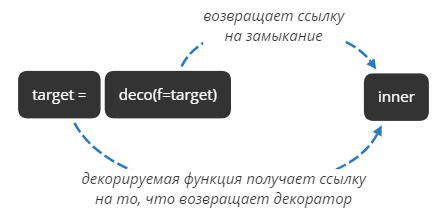
\includegraphics[scale=0.85]{figures/target_deco_formula.png}
	\caption{ К вопросу о механизме работы декоратора с вложенной функцией }\label{fig:target_deco_formula}
\end{figure}


\section{Замыкания/фабричные функции в \texttt{Python}}

Под термином \emph{замыкание} или \emph{фабричная функция} подразумевается объект функции, который сохраняет значения в \emph{объемлющих областях видимости}, даже когда эти области могут прекратить свое существование \cite[\strbook{488}]{lutz:learningpython-2011}.

В источнике \cite[\strbook{222}]{ramalho:python-2016} приводится несколько отличное определение\footnote{Определение содержит авторские правки}: \emph{замыкание} -- это вложенная функция с расширенной областью видимости, которая охватывает все \emph{неглобальные} переменные, объявленные в области видимости объемлющей функции, и способная работать с этими переменными даже после того как локальная область видимости объемлющей функции будет уничтожена.

Замыкания и вложенные функции особенно удобны, когда требуется реализовать концепцию отложенных вычислений \cite{beazley:python-2010}.

\remark{
Все же правильнее <<фабрикой функций>> называть всю конструкцию из объемлющей и вложенной функций, а <<замыканием>> -- только вложенную функцию
}

Рассмотрим в качестве примера следующую функцию

\begin{lstlisting}[
style = ironpython,
emph = {maker, action},
numbers = none
]
def maker(N):
    def action(X):
        return X**N  # функция action запоминает значение N в объемлющей области видимости
    return action
\end{lstlisting}

Здесь определяется внешняя функция, которая просто создает и возвращает вложенную функцию, не вызывая ее. Если вызвать внешнюю функцию

\begin{lstlisting}[
style = ironpython,
emph = {maker},
numbers = none
]
>>> f = maker(2)  # запишет 2 в N
>>> f  # <function action at 0x0147280>
\end{lstlisting}
она вернет ссылку на созданную ею вложенную функцию, созданную при выполнении вложенной инструкции \texttt{def}. Если теперь вызвать то, что было получено от внешней функции

\begin{lstlisting}[
style = ironpython,
numbers = none
]
>>> f(3)  # запишет 3 в X, в N по-прежнему хранится число 2
>>> f(4)  # 4**2
\end{lstlisting}
будет вызвана вложенная функция, с именем \texttt{action} внутри функции \texttt{maker}. Самое необычное здесь то, что вложенная функция продолжает хранить число 2, значение переменной \texttt{N} в функции \texttt{maker} даже при том, что к моменту вызова функции \texttt{action} функция \texttt{maker} уже \emph{завершила свою работу и вернула управление}.

Когда функция используется как вложенная, в замыкание включается все ее окружение, необходимое для работы внутренней функции \cite[\strbook{137}]{beazley:python-2010}.

\subsection{Области видимости и значения по умолчанию применительно к переменным цикла}

Существует одна известная особенность для функций или lambda-выражений: если lambda-выражение или инструкция \texttt{def} вложены в цикл внутри другой функции и вложенная функция ссылается на переменную из объемлющей области видимости, которая изменяется в цикле, все функции, созданные в этом цикле, будут иметь одно и то же значение -- значение, которое имела переменная на последней итерации \cite[\strbook{492}]{lutz:learningpython-2011}.

Например, ниже предпринята попытка создать список функций, каждая из которых запоминает текущее значение переменной \texttt{i} из объемлющей области видимости

\begin{lstlisting}[
title = {\sffamily Эта реализация работать НЕ будет},
style = ironpython,
emph = {makeActions},
numbers = none
]
def makeActions():
    acts = []
    for i in range(5):  # область видимости объемлющей функции
        acts.append(
            lambda x: i**x  # локальная область видимости вложенной анонимной функции
        ) 
    return acts
    
acts = makeActions()
print(acts[0](2))  # вернет 4**2, последнее значение i
print(acts[3](2))  # вернет 4**2, последнее значение i
\end{lstlisting}

Такой подход не дает желаемого результата, потому что поиск переменной в объемлющей области видимости производится позднее, \emph{при вызове вложенных функций}, в результате все они получат одно и то же значение (значение, которое имела переменная цикла на последней итерации).

Это один из случаев, когда необходимо явно сохранять значение из объемлющей области видимости в виде аргумента со значением по умолчанию вместо использования ссылки на переменную из объемлющей области видимости.

То есть, чтобы фрагмент заработал, необходимо передать текущее значение переменной из объемлющей области видимости в виде значения по умолчанию. Значения по умолчанию вычисляются в момент \emph{создания вложенной функции} (а не когда она \emph{вызывается}), поэтому каждая из них сохранит свое собственное значение \texttt{i}

\begin{lstlisting}[
title = {\sffamily Правильная реализация},
style = ironpython,
emph = {makeActions},
numbers = none
]
def makeActions():
    acts = []
    for i in range(5):
        acts.append(
            lambda x, i=i: i**x  # сохранить текущее значение i
        )
    return acts

acts = makeActions()
print(acts[0](2))  # вернет 0**2
print(acts[2](2))  # вернет 2**2
\end{lstlisting}

\quinta{%
Значения аргументов по умолчанию вложенных функций, динамически создаваемых в цикле на уровне области видимости объемлющей функции, вычисляются в момент \emph{создания} этих вложенных функций, а не в момент их вызова, поэтому \texttt{lambda x, i=i: ...} работает корректно
}

\section{Значения по умолчанию изменяемого типа данных в \texttt{Python}}

Если у функции есть аргумент, который получает ссылку на \emph{объект изменяемого типа данных} как на значение по умолчанию, то \emph{все вызовы функций} будут ссылаться на один и тот же изменяемый объект\footnote{По этой причине, как правило, только \emph{объекты неизменяемого типа данных} могут быть значениями по умолчанию. Если значение аргумента функции должно иметь возможность изменяться динамически, то этот аргумент функции инициализируют с помощью \texttt{None}, а затем передают ссылку на объект по условию} (идентификационный номер объекта не изменится).

Это удивляет. И когда говорят об аномальном поведении функции, аргумент которой ссылается на объект изменяемого типа данных, то обычно такое поведение объясняют следующим образом: значения аргументов по умолчанию вычисляются только один раз при загрузке модуля \cite[\strbook{77}]{slatkin:python-2016}. Однако такое объяснение не вскрывает механизм <<разделения>> ссылки между вызовами.

Лучше сказать так: если у функции есть аргумент, который ссылается на объект изменяемого типа данных, и в теле функции выполняется какая-то работа с этим изменяемым объектом (т.е. вносятся изменения в объект), то новые вызовы такой функции не сбрасывают значения по умолчанию до тех, которые были вычислены при загрузке модуля. Другими словами, если аргумент функции ссылается на объект изменяемого типа данных и над этим объектом выполняется какая-то работа в теле функции, то каждый новый вызов функции будет изменять этот изменяемый объект в \emph{определении} функции и потому каждый следующий вызов будет оперировать с уже измененным объектом изменяемого типа данных.

\remark{
Значения аргументов по умолчанию для избежания странного поведения функции должны ссылаться на \emph{объекты неизменяемого типа данных}
}

\section{Калибровка классификаторов}

Подробности в статье А. Дьяконова \href{https://dyakonov.org/2020/03/27/%D0%BF%D1%80%D0%BE%D0%B1%D0%BB%D0%B5%D0%BC%D0%B0-%D0%BA%D0%B0%D0%BB%D0%B8%D0%B1%D1%80%D0%BE%D0%B2%D0%BA%D0%B8-%D1%83%D0%B2%D0%B5%D1%80%D0%B5%D0%BD%D0%BD%D0%BE%D1%81%D1%82%D0%B8/}{<<Проблема калибровки уверенности>>}.
\vspace{2mm}

Ниже описываются способы оценить качество калибровки алгоритма. Надо сравнить \emph{уверенность} (confidence) и \emph{долю верных ответов} (accuracy) на тестовой выборке.

Если классификатор <<хорошо откалиброван>> и для большой группы объектов этот классификатор возвращает вероятность принадлежности к положительному классу 0.8, то среди этих объектов будет приблизительно 80\% объектов, которые в действительности принадлежат положительному классу. То есть, если для группы точек данных общим числом 100 классификатор возвращает вероятность положительного класса 0.8, то приблизительно 80 точек на самом деле будут принадлежать положительному классу и доля верных ответов тогда составит 0.8.

\subsection{Непараметрический метод гистограммной калибровки (Histogram Binning)}

Изначально в методе использовались бины одинаковой ширины, но можно использовать и равномощные бины.

Недостатки подхода:

\begin{itemize}
	\item число бинов задается наперед,
	
	\item функция деформации не непрерывна,
	
	\item в <<равноширинном варианте>> в некоторых бинах может содержаться недостаточное число точек.
\end{itemize}

Метод был предложен Zadrozny В. и Elkan C. \href{http://cseweb.ucsd.edu/~elkan/calibrated.pdf}{\ttfamily Obtaining  calibrated  probability  estimates  from  decision  trees  and naive bayesian classifiers}.

\subsection{Непараметрический метод изотонической регрессии (Isotonic Regression)}

Строится монотонно неубывающая функция деформации оценок алгоритма.

Метод был предложен Zadrozny B. и Elkan C. \href{http://citeseerx.ist.psu.edu/viewdoc/download?doi=10.1.1.13.7457&rep=rep1&type=pdf}{\ttfamily Transforming classifier scores into accurate multiclass probability estimates}.

Функция деформации по-прежнему не является непрерывной.

\subsection{Параметрическая калибровка Платта (Platt calibration)}

Изначально этот метод калибровки разрабатывался только для метода опорных векторов, оценки которого лежат на вещественной оси (по сути, это расстояния до оптимальной разделяющей классы прямой, взятые с нужным знаком). Считается, что этот метод не очень подходит для других моделей.

Предложен Platt~J. \href{http://citeseerx.ist.psu.edu/viewdoc/download;jsessionid=EA4888FEE74FB677B492740F59CDFE1F?doi=10.1.1.41.1639&rep=rep1&type=pdf}{\ttfamily Probabilistic  outputs  for  support  vector machines and comparisons to regularized likelihood methods}.

\subsection{Логистическая регрессия в пространстве логитов}

\subsection{Деревья калибровки}

Стандартный алгоритм строит строит суперпозицию дерева решений на исходных признаках и логистических регрессий (каждая в своем листе) над оценками алгоритма:

\begin{itemize}
	\item Построить на исходных признаках решающее дерево (не очень глубокое),
	
	\item В каждом листе -- обучить логистическую регрессию на одном признаке,
	
	\item Подрезать дерево, минимизируя ошибку.
\end{itemize}

\subsection{Температурное шкалирование (Temperature Scaling)}

Этот метод относится к классу DL-методов калибровки, так как он был разработан именно для калибровки нейронных сетей. Метод представляет собой простое многомерное обобщение шкалирования Платта.

\section{Приемы работы с менеджером пакетов \texttt{conda}}

\subsection{Создание виртуального окружения}

Создать виртуальное окружение \texttt{dashenv}

\begin{lstlisting}[
numbers = none
]
conda create --name dashenv
\end{lstlisting}

Создать виртуальное окружение с указанием версии \texttt{Python}

\begin{lstlisting}[
numbers = none
]
conda create --name testenv python=3.6
\end{lstlisting}

Создать виртуальное окружение с указанием пакета

\begin{lstlisting}[
numbers = none
]
conda create --name testenv scipy
\end{lstlisting}

Создать виртуальное окружение с указанием версии \texttt{Python} и нескольких пакетов

\begin{lstlisting}[
numbers = none
]
conda create --name testenv python=3.6 scipy=0.15.0 astroid babel
\end{lstlisting}

\remark{%
Рекомендуется устанавливать сразу несколько пакетов, чтобы избежать конфликта зависимостей
}

Для того чтобы при создании нового виртуального окружения не требовалось каждый раз устанавливать базовые пакеты, которые обычно используются в работе, можно привести их список в конфигурационном файле \texttt{.condarc} в разделе \texttt{create\_default\_packages}

\begin{lstlisting}[
title = {\sffamily .condarc},
numbers = none
]
ssl_verify: true
channels:
 - conda-forge
 - defaults
report_errors: true
default_python:
create_default_packages:
 - matplotlib
 - numpy
 - scipy
 - pandas
 - seaborn
\end{lstlisting}

Если для текущего виртуального окружения не требуется устанавливать пакеты из набора по умолчанию, то при создании виртуального окружения следует указать специальный флаг
\lstinline{--no-default-packages}

\begin{lstlisting}[
numbers = none
]
conda create --no-default-packages --name testenv python
\end{lstlisting}

Создать виртуальное окружение можно и из файла \texttt{environment.yml} (первая строка этого файла станет именем виртуального окружения)

\begin{lstlisting}[
title = {\sffamily environment.yml},
numbers = none
]
name: stats2
channels:
 - conda-forge
 - defaults
dependencies:
 - python=3.6   # or 2.7
 - bokeh=0.9.2
 - numpy=1.9.*
 - nodejs=0.10.*
 - flask
 - pip:
  - Flask-Testing
\end{lstlisting}

\begin{lstlisting}[
numbers = none
]
conda env create -f environment.yml
\end{lstlisting}

При создании виртуального окружения можно указать путь до целевой директории, где будут размещаться файлы окружения. Следующая команда создаст виртуальное окружение в поддиректории текущей рабочей директории \texttt{envs}\footnote{В данном случае чтобы удалить виртуальную среду достачно просто удалить директорию \texttt{envs}}

\begin{lstlisting}[
numbers = none
]
conda create --prefix ./envs jupyterlab matplotlib
\end{lstlisting}

С помощью файла спецификации можно создать \emph{идентичное виртуальное окружение} (i) на той же платформе операционной системы, (ii) на той же машине, (iii) на какой-либо другой машине (перенести настройки окружения).

Для этого предварительно требуется создать собственно файл спецификации

\begin{lstlisting}[
numbers = none
]
conda list --explicit > spec-file.txt
\end{lstlisting}

Имя файла спецификации может быть любым. Файл спецификации обычно не является кросс-платформенным и поэтому имеет комментарий в верхней части файла (\lstinline{#platform: osx-64}), указывающий платформу, на которой он был создан.

Теперь для того чтобы \emph{создать} окружение достаточно воспользоваться командой

\begin{lstlisting}[
numbers = none
]
conda create --name myenv --file spec-file.txt
\end{lstlisting}

Файл спецификации можно использовать для установки пакетов в существующее окружение

\begin{lstlisting}[
numbers = none
]
conda install --name myenv --file spec-file.txt
\end{lstlisting}


\subsection{Активация/деактивация виртуального окружения}

Активировать виртуальное окружение \texttt{dashenv}

\begin{lstlisting}[
numbers = none
]
conda activate dashenv
\end{lstlisting}

Активировать виртуальное окружение в случае, когда оно создавалось с \lstinline{--prefix}, можно указав полный путь до окружения
\begin{lstlisting}[
numbers = none
]
conda activate E:\[WorkDirectory]\[Python_projects]\directory_for_experiments\envs
\end{lstlisting}

В этом случае в строке приглашения командной оболочки по умолчанию будет отображаться полный путь до окружения. Чтобы заменить длинный префикс в имени окружения на более удобный псевдоним достаточно использовать конструкцию

\begin{lstlisting}[
numbers = none
]
conda config --set env_prompt ({name})
\end{lstlisting}
которая добавит в конфигурационный файл \texttt{.condarc} следующую строку

\begin{lstlisting}[
title = {\sffamily .condarc},
numbers = none
]
...
env_prompt: ({name})
\end{lstlisting}
и теперь имя окружения будет \texttt{(envs)}.

Деактивировать виртуальное окружение

\begin{lstlisting}[
numbers = none
]
conda deactivate
\end{lstlisting}

\subsection{Обновление виртуального окружения}

Обновить виртуальное окружение может потребоваться в следующих случаях:

\begin{itemize}
	\item обновилась одна из ключевых зависимостей,
	
	\item требуется добавить пакет (добавление зависимости),
	
	\item требуется добавить один пакет и удалить другой.
\end{itemize}

В любом из этих случаев все что нужно для того чтобы обновить виртуальное окружение это просто обновить файл \texttt{environment.yml}\footnote{Этот файл должен находится в той же директории что и директория окружения \texttt{envs}}, а затем запустить команду

\begin{lstlisting}[
numbers = none
]
conda env update --prefix ./envs --file environment.yml --prune
\end{lstlisting}

Опция \lstinline{--prune} приводит к тому, что \texttt{conda} удаляет все зависимости, которые больше не нужны для окружения.

\subsection{Вывод информации о виртуальном окружении}

Вывести список доступных виртуальных окружений

\begin{lstlisting}[
numbers = none
]
conda env list
\end{lstlisting}

Вывести список пакетов, установленных в указанном окружении

\begin{lstlisting}[
numbers = none
]
conda list --name myenv
\end{lstlisting}

Вывести информацию по конкретному пакету указанного окружения

\begin{lstlisting}[
numbers = none
]
conda list --name dashenv matplotlib
\end{lstlisting}


\subsection{Удаление виртуального окружения}

Удалить виртуальное окружение \texttt{heroku\_env}

\begin{lstlisting}[
numbers = none
]
conda env remove --name heroku_env
\end{lstlisting}

\subsection{Экспорт виртуального окружения в \texttt{environment.yml}}

Экспортировать активное виртуальное окружение в yml-файл

\begin{lstlisting}[
numbers = none
]
conda env export > environment.yml
\end{lstlisting}


\section{Инструмент автоматического построения дерева проекта под задачи машинного обучения}

Для автоматизации построения типового (или кастомизированного) дерева проекта по машинному обучению и анализу данных удобно использовать \href{https://cookiecutter.readthedocs.io/en/1.7.2/README.html}{\texttt{cookicutter}}.

На операционную систему под управлением \texttt{Windows} \texttt{cookicutter} можно установить с помощью менеджера пакетов \texttt{pip}

\begin{lstlisting}[
numbers = none
]
pip install cookiecutter
\end{lstlisting} 
а на операционную систему под управлением \texttt{MacOS X} с помощью менеджера \texttt{brew}

\begin{lstlisting}[
numbers = none
]
brew install cookiecutter
\end{lstlisting}

В самом простом случае \texttt{cookicutter} можно использовать как утилиту командной строки. Например для того чтобы создать проект по шаблону для задач машинного обучения достаточно сделать следующее

\begin{lstlisting}[
style = ironpython,
numbers = none,
]
cookiecutter https://github.com/drivendata/cookiecutter-data-science
\end{lstlisting}

Утилита предложит ответить на несколько вопросов (название репозитория, имя автора и т.д.), а затем создаст дерево проекта.

\section{Управление локальными переменными окружения проекта}

Для того чтобы создать \emph{локальные переменные проекта}\footnote{То есть переменные, привязанные к текущему проекту} достаточно разместить пары вида <<ключ=значение>> в файле \texttt{.env}, а затем прочитать его с помощью специальной библиотеки \texttt{dotenv} \url{https://pypi.org/project/python-dotenv/}. Например

\begin{lstlisting}[
style = ironpython,
numbers = none
]
#.env в текущей директории проекта
EMAIL = leor.finkelberg@yandex.ru
POSTGRESQL_PASSWORD = Evdimonia
\end{lstlisting}

\begin{lstlisting}[
style = ironpython,
numbers = none
]
import os
from pathlib import Path
from dotenv import load_dotenv

dotenv_path = Path(__file__).resolve().parents[0].joinpath('.env')
print(f'[INFO] path: {dotenv_path}')  # [INFO] path: E:\[WorkDirectory]\[Python_projects]\directory_for_experiments\.env

load_dotenv(dotenv_path)  # загрузить .env

# извлекать значения локальных переменных окружения проекта можно с помощью `os.getenv(key)`
# или `os.environ.get(key)`
for key in (s.upper() for s in ('email', 'postgresql_password')):
    print('[INFO] from file `.env`({}) -> {}'.format(key, os.getenv(key)))
\end{lstlisting}

\section{Приемы работы с модулем \texttt{subprocess}}

Ниже приводится пример использования модуля \texttt{subprocess} для отыскания самого большого файла в \texttt{git}-репозитории
\begin{lstlisting}[
style = ironpython,
emph = {popen_2_str},
numbers = none
]
import os
import subprocess
import pathlib
from subprocess import Popen, PIPE, STDOUT

# --- объявление функций: begin
def popen_2_str(cmd: str, shell=True, universal_newlines=True, stdout=PIPE) -> str:
    return Popen(cmd, shell=shell,
                 universal_newlines=universal_newlines,
                 stdout=stdout).stdout.read().strip()

def stat(filename):
    res = popen_2_str(f"stat {filename}")
    print(f'>>> Statistic:\n{res}')

def summary(commits):
    print(f'### Summary ({__file__}) ###:\n>>> idx-file name: {idx_file}'
          f'\n>>> SHA blob: {shablob}\n>>> Commits:')
    print(commits)
# --- объявление функций: end

GIT_PATH = pathlib.Path('.git/objects/pack/')

# тоже самое что и `git gc &> /dev/null`
exit_code = subprocess.call("git gc", shell=True,
                            stdout=open(os.devnull, 'w'), stderr=STDOUT)

if not exit_code:
    # возвращает имя idx-файла
    idx_file = popen_2_str(f"ls -l {GIT_PATH} | grep -iE '*.idx' "
                           f"| awk -F ' ' '{{ print $9 }}'")
    # возвращает абсолютный путь до idx-файла
    abs_path_idx_file = pathlib.Path.joinpath(GIT_PATH, idx_file)
    if os.path.exists(abs_path_idx_file):
    # возвращает SHA <<большого>> файла
        shablob = popen_2_str(f"git verify-pack -v {abs_path_idx_file} | sort -k 3 -n "
                              f"| tail -n 1 | awk -F ' ' '{{ print $1 }}'")
        # возвращает имя файла по его SHA
        filename = popen_2_str(f"git rev-list --objects --all | grep {shablob} "
                               f"| awk -F ' ' '{{ print $2 }}'")
        # возвращает коммиты, связанные с данным файлом
        commits = popen_2_str(f"git log --oneline -- {filename}")
        summary(commits)
        stat(filename)
    else:
        print(f"File {abs_path_idx_file} not found...")
else:
    print('Something went wrong.')
\end{lstlisting}

\section{Решающие деревья и сопряженные вопросы}

\subsection{Коэффициент Джини}

\emph{Коэффициент Джини}\footnote{Еще говорят индекс Джини или загрязненность Джини} (Gini impurity) это просто вероятность неверной маркировки в узле случайно выбранного образца (для чистых листьев коэффициент Джини равен 0)
\begin{align}
	I_G(n) = 1 - \sum_{i=1}^{J}p_i^2,
\end{align}
где $ p_i $ -- частоты представителей разных классов в листе дерева.

К примеру, если решается задача бинарной классификации ($ J = 2 $) на выборке из 6 объектов и в данном расщеплении в один класс попали 2 объекта, а в другой 4, то индекс Джини будет равен
\begin{align}
	I_G(n)=1 - \left( \left( \frac{2}{6} \right)^2 + \left( \frac{4}{6} \right)^2 \right) = 0,444.
\end{align}

\subsection{Случайный лес}

Случайный лес -- это модель, представляющая ансамбль решающих деревьев, дополненная двумя концепциями:
\begin{itemize}
	\item концепцией бутрстапированных выборок,
	
	\item концепцией случайных подпространств.
\end{itemize}

Хотя каждое решающее дерево может иметь большой разброс по отношению к определенному набору тренировочных данных, обучение деревьев на разных наборах образцов позволяет снизить общий разброс леса.


\section{Анализ временных рядов}

\subsection{Прогнозирование временных рядов. Метод имитированных исторических прогнозов}

При разбиении данных на обучающую и проверочную выборки важно помнить о том, как модель в итоге будет использоваться на практике. Так, при выполнении предсказаний для той же генеральной совокупности, из которой получены исходные данные (\emph{интерполяция}), достаточным может оказаться простое случайное разбиение данных. В случаях же, когда модель предназначена для прогнозирования будущего (\emph{экстраполяция}), более точную оценку ее предсказательных свойств можно получить только если проверочная выборка содержит данные из будущего (например, если исходные данные охватывают период в два года, то модель можно было бы обучить на данных первого года, а затем проверить ее обобщающую способность на данных второго года).

Стандартным методом оценки качества нескольких альтернативных моделей является перекрестная проверка. Суть этого метода сводится к тому, что исходные обучающие данные случайным образом разбиваются на $ k $ блоков, после чего модель $ k $ раз обучается на $ k - 1 $ блоках, а оставшийся блок каждый раз используется для проверки качества предсказаний на основе той или иной подходящей случаю метрики. Полученная таким образом средняя метрика будет хорошей оценкой качества предсказаний модели на новых данных.

К сожалению, в случае с моделями временных рядов такой способ выполнения перекрестной проверки будет бессмысленным и не отвечающим стоящей задаче. Поскольку во временных рядах, как правило, имеет место тесная корреляция между близко расположенными наблюдениями, мы не можем просто разбить такой ряд случайным образом на $ k $ частей -- это приведет к потере указанной корреляции. Более того, в результате случайного разбиения данных на несколько блоков может получиться так, что в какой-то из итераций мы построим модель преимущественно по недавним наблюдениям, а затем оценим ее качество на блоке из давних наблюдений. Другими словами, мы построим модель, которая будет предсказывать прошлое, что не имеет никакого смысла -- ведь мы пытаемся решить задачу по предсказаним будущего.

Для решения описанной проблемы при работе с временными рядами применяют несколько модификаций перекрестной проверки. Например, в пакете Prophet, реализован так называемый метод <<имитированных исторических прогнозов>> (simulated historical forecast).

Метод имитированных исторических прогнозов \url{https://r-analytics.blogspot.com/2019/10/prophet-shf.html}. Для создания модели временного ряда мы используем данные за определенный исторический отрезок времени. Далее по полученной модели рассчитываются прогнозные значения для некоторого интересующего нас промежутка времени (горизонта прогноза) в будущем. Такая процедура повторяется каждый раз, когда необходимо сделать новый прогноз.

В пределах отрезка с исходными обучающими данными выбирают $ k $ точек отсчета (в терминологии Prophet), на основе которых формируются блоки данных для выполнения перекрестной проверки: все исторические наблюдения, предшествующие $ k $-ой точке отсчета (а также сама эта точка), образуют обучающие данные для подгонки соответствующей модели, а $ H $ исторических наблюдений, следующих за точкой отсчета, образуют \emph{прогнозный горизонт}. Расстояние между точками отсчета называется периодом и по умолчанию составляет $ H/2 $. Обучающие наблюдения в первом из $ k $ блоков образуют так называемый начальный отрезок. В Prophet длина этого отрезка по умолчанию составляет $ 3\,H $, однако этот параметр можно изменить.

Каждый раз после подгонки модели на обучающих данных из $ k $-ого блока рассчитываются предсказания для прогнозного горизонта того же блока, что позволяет оценить качество прогноза с помощью подходящей метрики. Значения этой метрики, усредненные по каждой дате прогнозных горизонтов каждого блока, в итоге дают оценку качества предсказаний, которую можно ожидать от модели, построенной \emph{по всем исходным обучающим данным}.

\subsection{Обнаружение аномалий во временных рядах}

Обнаружение аномалий относится к поиску непредвиденных значений (паттернов) в потоках данных. Аномалия (выброс, ошибка, отклонение или исключение) -- это отклонение поведение системы от стандартного (ожидаемого).

Аномалии могут возникать в данных самой различной природы и структуры в результате технических сбоев, аварий, преднамеренных взломов и т.д.

Аномалии в данных могут быть отнесены к одному из трех основных типов \cite{chandola:2009}:
\begin{itemize}
	\item \emph{Точечные аномалии}: возникают в ситуации, когда отдельный экземпляр данных может рассматриваться как аномальный по отношению к остальным данным; большинство существующих методов создано для распознавания точечных аномалий,
	
	\item \emph{Контекстуальные аномалии}: наблюдаются, если экземпляр данных является аномальным лишь в определенном контексте (данный вид аномалий также называется условным)
	
	\begin{itemize}
		\item контекстуальные атрибуты используются для определения контекста (или окружения) для каждого экземпляра; во временных рядах контекстуальным атрибутом является время, которое определяет положение экземпляра в целой последовательности; контекстуальным атрибутом также может быть положение в пространстве или более сложные комбинации свойств,
		
		\item поведенческие атрибуты определяют не контекстуальные характеристики, относящиеся к конкретному экземпляру данных,
	\end{itemize}
	
	\item \emph{Коллективные аномалии}: возникают, когда последовательность связанных экземпляров данных (например, фрагмент временного ряда) является аномальной по отношению к целому набору данных. Отдельный экземпляр данных в такой последовательности может не являться отклонением, однако совместное появление таких экземляров является коллективной аномалией; кроме того, если точечные или контекстуальные аномалии могут наблюдаться в любом наборе данных, то коллективные наблюдаются только в тех, где данные связанны между собой.
\end{itemize}

Часто для решения задачи поиска аномалий требуется набор данных, описывающих систему. Каждый экземпляр в нем описывается меткой, указывающей, является ли он нормальным или аномальным. Таким образом, множество экземпляров с одинаковой меткой формируют соответствующий класс. 

Создание подобной промаркированной выборки обычно проводится вручную и является трудоемким и дорогостоящим процессом. В некоторых случаях получить экземпляры аномального класса невозможно в силу отсутствия данных и возможных отклонениях в системе, в других могут отсутствовать метки обоих классов. В зависимости от того, какие классы данных используются для реализации алгоритма, методы поиска аномалий могут выполняться в одном из трех перечисленных режимов:
\begin{itemize}
	\item \textbf{Режим распознавания с учителем}. Данная методика требует наличия обучающей выборки, полноценно представляющей систему и включающей экземпляры данных нормального и аномального классов. Работа алгоритма происходит в два этапа: обучение и распознование. На первом этапе строится модель, с которой в последствии сравниваются экземпляры, не имеющие метки. В большинстве случаев предполагается, что \emph{данные} \emph{не меняют свои статистические характеристики}, иначе возникает необходимость изменять классификатор. Основной сложностью алгоритмов, работающих в режиме распознования с учителем, является формирование данных для обучения. Часто аномальный класс представлен значительно меньшим числом экземпляров, чем нормальный, что может приводить к неточностям в полученной модели. В таких случаях применяется \emph{искусственная генерация аномалий}.
	
	\textbf{Режим распознования частично с учителем}. Исходные данные при этом подходе представляют только нормальный класс. Обучившись на одном классе, система может определять принадлежность новых данных к нему, таким образом, определяя противоположенный. Алгоритмы, работающие в режиме распознования частично с учителем, не требуют информации об аномальном классе экземпляров, вследствие чего они шире применимы и позволяют распознавать отклонения в отсутствие заранее определенной информации о них.
	
	\textbf{Режим распознавания без учителя}. Применяется при отсутствии априорной информации о данных. Алгоритмы распознавания в режиме без учителя базируются на предположении о том, что аномальные экземпляры встречаются гораздо реже нормальных. Данные обрабатываются, наиболее отдаленные определяются как аномалии. Для применения этой методики должен быть доступен весь набор данных, т.е. она не может применяться в режиме реального времени.
\end{itemize}

Метод опорных векторов\footnote{В \texttt{sklearn} есть реализация одноклассового метда опорных векторов \href{https://scikit-learn.org/stable/modules/generated/sklearn.svm.OneClassSVM.html}{\ttfamily OneClassSVM} (позволяет задать долю аномальных объектов в выборке с помощью параметра \texttt{nu})} применяется для поиска аномалий в системах, где нормальное поведение представляется только одним классом. Данный метод определяет границу региона, в котором находятся экземпляры нормальных данных. Для каждого исследуемого экземпляра определяется, находится ли он в определенном регионе. Если экземпляр оказывается вне региона, он определяется как аномальный.

Пример использования одноклассового метода опорных векторов
\begin{lstlisting}[
style = ironpython,
emph = {transform_to_zero_minus_one},
numbers = none
]
import numpy as np
import matplotlib.pyplot as plt
from sklearn.svm import OneClassSVM


def transform_to_zero_minus_one(arr):
    return np.where(arr < 0, arr, 0)

N = 250  # длина временного ряда
scale = 50  # масштаб меток для графика аномалий

# подготавливаем тренировочный и тестовый набор данных
data_train = np.random.RandomState(42).randn(N)
data_test = np.random.RandomState(2).randn(int(0.1*N))
data_train[[40, 50, 80]] *= 100
data_test[[2, 5]] *= 50

# обучаем классификатор и готовим предсказания
clf = OneClassSVM(nu=0.03).fit(data_train.reshape(-1, 1))
predicted_anomalies = clf.predict(data_test.reshape(-1, 1))

plt.plot(data_test,
    marker = '.',
    markersize = 12,
    markerfacecolor = 'w',
    color = 'k',
    label='тестовый набор данных')

plt.bar(np.arange(0, data_test.shape[0]),
    transform_to_zero_minus_one(predicted_anomalies)*scale,
    alpha = 0.5,
    color = 'b',
    label='аномалии')
plt.legend()
\end{lstlisting}

\begin{figure}[h]
	\centering
	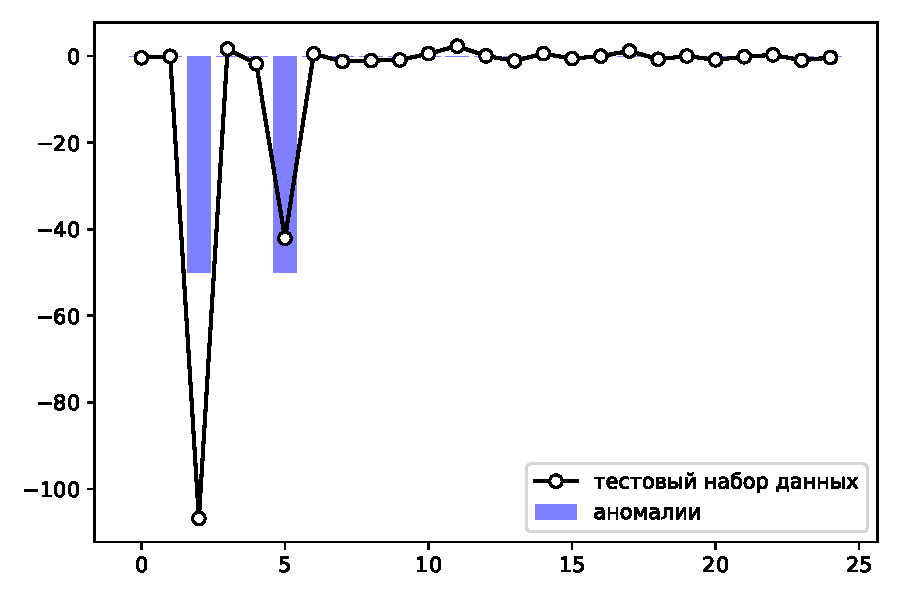
\includegraphics[scale=0.55]{figures/oneclasssvm_test.pdf}
	\caption{ Пример детектирования аномалий на тестовой наборе данных }\label{fig:oneclasssvm}
\end{figure}

Кластеризация. Данная методика предполагает группировку похожих экземпляров в кластеры и не требует знаний о свойствах возможных отклонений: нормальные данные образуют большие плотные кластеры, а аномальные -- маленькие и разрозненные. Одной из простейших реализацией подхода на основе кластеризации является алгоритм метода $ k $-средних.

При использовании методов статистического анализа исследуется процесс, строится его профиль (статистическая модель), которые затем сравнивается с реальным поведением. Если разница в реальном и предполагаемом поведении системы, определяется заданной функцией аномальности, выше установленного порога, делается вывод о наличии отклонений. Применяется предположении о том, что нормальное поведение системы будет находиться в зоне высокой вероятности, в то время как выбросы -- в зоне низкой.

Данный класс методов удобен тем, что не требует заранее определенных знаний о виде аномалии. Однако сложности могут возникать в определении точного статистического распределения и порога.

Методы статистического анализа подразделяются на две группы:
\begin{itemize}
	\item \emph{Параметрические методы}. Предполагают, что нормальные данные генерируются параметрическим распределением с параметрами $ \theta $ и функцией плотности вероятности $ \mathbb{P}(x, \theta) $, где $ x $ -- наблюдение. Аномалия является обратной функцией распределения. Эти методы часто основываются на Гауссовской или регрессионной модели, а также их комбинации.
	
	\item Непараметрические методы. Предполагается, что структура модели не определена априорно, вместо этого она определяется из предоставленных данных. Включает методы на основе гистограмм или функции ядра.
\end{itemize}

Базовый алгоритм поиска аномалий с применением гистограмм включает два этапа. На первом этапе происходит построение гистограммы на основе различных значений выбранной характеристики для экземпляров тренировочных данных. На втором этапе для каждого из исследуемых экземпляров определяется принадлежность к одному из столбцов гистограммы. Не принадлежащие ни к одному из столбцов экземпляры помечаются как аномальные.

Алгоритм ближайшего соседа. Для использования данной методики необходимо определить понятие расстояния (меры похожести) между объектами. Примером может быть евклидово расстояние.

Два основных подхода основаваются на следующих предположениях:
\begin{itemize}
	\item Расстояние до $ k $-ого ближайшего соседа. Для реализации этого подхода расстояние до ближайшего объекта определяется для каждого тестируемого экземпляра класса. Экземпляр, являющийся выбросом, наиболее отдален от ближайшего соседа.
	
	\item Использование относительной плотности основано на оценке плотности окрестности каждого экземпляра данных. Экземпляр, который находится в окрестности с низкой плотностью, оценивается как аномальный, в то время как экземпляр в окрестности с высокой плотностью оценивается как нормальный. Для данного экземпляра данных расстояние до его $ k $-ого ближайшего соседа эквивалентно радиусу гиперсферы с центром в данном экземпляре и содержащей $ k $ остальных экземпляров.
\end{itemize}

Выявление аномалий в режиме реального времени может потребовать дополнительной модификации методов. Наиболее простым в реализации является \emph{алгоритм скользящего окна}.

Данная методика используется для временных рядов, которые разбиваются на некоторое число последовательностей -- окон. Необходимо выбрать окно фиксированной длины, меньшей чем длина самого временного ряда, чтобы захватить аномалию в процессе скольжения. Поиск аномальной последовательности осуществляется при помощи скольжения окна по всему ряду с шагом, меньшим длины окна.




\subsection{Приемы работы с библиотекой \texttt{Prophet}}

Установить библиотеку можно с помощью менеджера пакетов \texttt{conda}
\begin{lstlisting}[
style = cmd,
numbers = none
]
conda install -c conda-forge fbprophet
\end{lstlisting}

\texttt{Prophet} была разработана для прогнозирования большого числа различных бизнес-показателей и строит неплохие baseline-прогнозы.

По сути Prophet-модель представляет собой аддитивную регрессионную модель
\begin{align*}
	y(t) = g(t) + s(t) + h(t) + \varepsilon_t,
\end{align*}
где $ g(t) $ -- тренд (может быть представлен \emph{кусочно-линейной} или \emph{логистической функцией}\footnote{Логистическая функция удобна для моделирования роста с насыщением, когда при увеличении показателя снижается темп его роста}); $ s(t) $ -- сезонная компонента, отвечающая за периодические/квазипериодические изменения, связанные с \emph{недельной} и \emph{годовой сезонностью}\footnote{Моделируется с помощью рядов Фурье}; $ h(t) $ -- отвечает за аномальные дни (праздники, Black Fridays и т.д.); $ \varepsilon $ -- содержит информацию, которая не учтена моделью.

Подробнее о математической стороне вопроса рассказывается в статье \url{https://peerj.com/preprints/3190/}. К слову, в этой статье качество моделей оценивается с помощью MAPE и MAE. MAPE (mean absolute percentage error) -- это средняя абсолютная ошибка нашего прогноза. Пусть $ y_i $ -- значение целевого вектора, а $ \hat{y}_i $ -- это соответствующий этой величине прогноз модели. Тогда $ \varepsilon_i = y_i - \hat{y}_i $ -- это ошибка прогноза, а $ p_i = \frac{\varepsilon_i}{y_i} $ -- относительная ошибка прогноза.

Таким образом средняя абсолютная ошибка выражается следующей формулой
$$
MAPE = \frac{1}{N}\sum_{i = 1}^{N} |p_i|.
$$

MAPE часто используется для оценки качества, поскольку эта величина относительная и по ней можно сравнивать качество даже на различных наборах данных.

Библиотека \texttt{Prophet} имеет интерфейс, похожий на интерфейс \texttt{sklearn}: сначала мы создаем модель, затем вызываем у нее метод \texttt{fit} и затем получаем прогноз. На вход метод \texttt{fit} получает объект DataFrame с двумя столбцами: \texttt{ds} -- временная метка (поле должно иметь тип \texttt{date} или \texttt{timestamp}), и целевой показатель \texttt{y}.

Разработчики рекомендуют делать предсказания по нескольким месяцам данных (в идеале год и более).

Пример
\begin{lstlisting}[
style = ironpython,
numbers = none
]
import fbprophet
from fbprophet.plot import add_changepoints_to_plot
import pandas as pd
import matplotlib.pyplot as plt


data_all = pd.read_csv('AirPassengers.csv')
# в наборе данных, на котором обучается модель обязательно должны быть столбцы `ds` и `y`
data_all = data_all.rename(columns={ 'Month' : 'ds', 'Passengers' : 'y' })
data_all['ds'] = pd.to_datetime(data_all['ds'])
M = 100
data_train = data_all[:M]  # обучающий набор данных
data_test = data_all[M:]   # тестовый набор данных

model = fbprophet.Prophet(
    changepoint_prior_scale=0.035,
    weekly_seasonality=True,
    yearly_seasonality=True,
    seasonality_mode='multiplicative'
)
model.fit(data_train)  # обучение модели

future_points = data_test.shape[0]  # число точек прогнозного горизонта
# преобразование в точек в метки, имеющие смысл времени
time_points_for_predict = model.make_future_dataframe(future_points, freq='M')
forecast = model.predict(time_points_for_predict)  # прогноз

fig, ax = plt.subplots(figsize=(8, 4))
plt.plot(data_train['ds'], data_train['y'], marker='.', label='Train data')
plt.plot(data_test['ds'], data_test['y'], marker='.', color='k', label='Test data')
plt.plot(forecast['ds'][M:], forecast['yhat'][M:], marker='.', color='r', label='Predict')
plt.axvspan(forecast['ds'][M],forecast['ds'][M+43], facecolor='grey', alpha=0.25)
plt.legend()
# добавить точки перегиба
a = add_changepoints_to_plot(fig.gca(), model, forecast)
\end{lstlisting}

С помощью конструкции \lstinline{model.plot_components(forecast);} можно посмотреть компоненты временного ряда (тренд, недельную и годовую сезонность).

\begin{figure}[h]
	\centering
	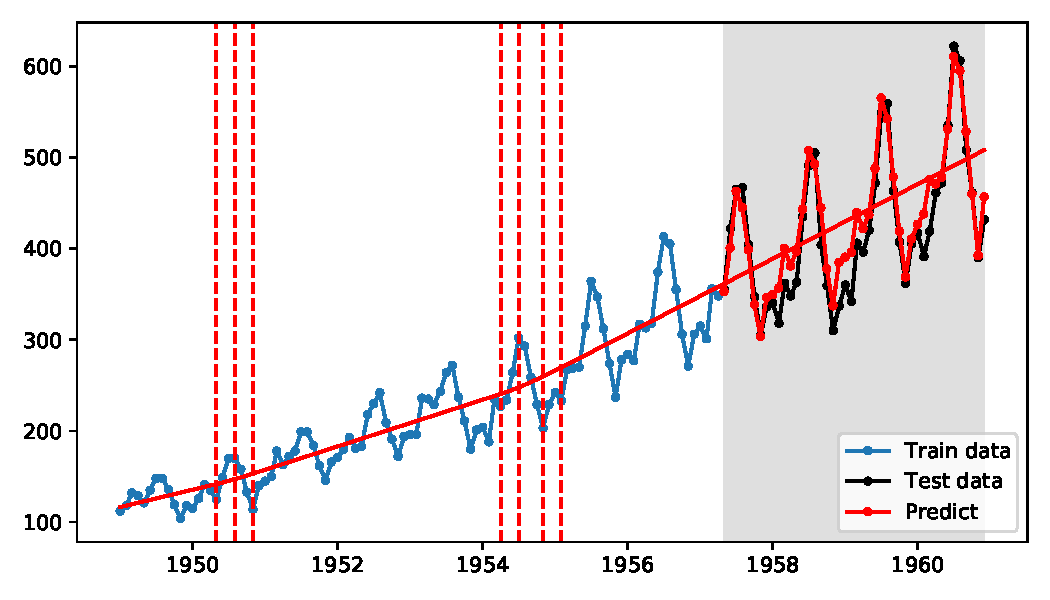
\includegraphics[scale=0.65]{figures/prophet_test.pdf}
	\caption{Пример использования библиотеки \texttt{fbprophet}}}\label{fig:prophet_test}
\end{figure}

С помощью библиотеки \texttt{Prophet} можно учитывать эффекты <<праздников>>. Под термином <<праздник>> здесь понимается как <<настоящие>> официальные праздничные и выходные дни (например, Новый Год, Рождество и пр.), так и другие события, во время которых свойства моделируемой зависимой переменной существенно изменяются (спортивные или культурные мероприятия, природные явления и пр.).

Для добавления эффектов <<праздников>> в Prophet-модель необходимо сначала создать отдельную таблицу, содержащую как минимум два обязательных столбца: \texttt{holiday} и \texttt{ds}. Важно, чтобы эта таблица охватывала как исторический период, на основе которого происходит обучение модели, так и период в будущем, для которого необходимо сделать прогноз. Например, если какое-то важное событие встречается в обучающих данных, то его следует указать и для прогнозного периода (при условии, конечно, что мы ожидаем повторение этого события в будущем, и что дата этого события входит в прогнозный период).

Параметры класса \texttt{Prophet}:
\begin{itemize}
	\item \texttt{growth}: тип тренда. Принимает два возможных значения: linear и logistic,
	
	\item \texttt{changepoints}: список временных меток, соответствующих точкам излома тренда (т.е. датам, когда, как предполагается, произошли существенные изменения в тренде временного ряда). Если этот список не задан, то такие точки излома будут вычисляться автоматически,
	
	\item \texttt{n\_changepoints}: предполагаемое количество, точек излома (по умолчанию 25). Если параметр \texttt{changepoints} задан, то параметр \texttt{n\_changepoints} будет проигнорирован. Если же \texttt{changepoints} не задан, то \texttt{n\_changepoints} потенциальных точек излома будут распределены равномерно в предалах исторического отрезка, заданного параметром \texttt{changepoint\_range},
	
	\item \texttt{changepoint\_range}: доля исторических данных (начиная с самого первого наблюдения), в пределах которых будут оценены точки излома. По умолчанию составляет 0.8 (т.е. 80\% наблюдений),
	
	\item \texttt{yearly\_seasonality}: параметр настройки годовой сезонности (т.е. закономерных колебаний в пределах года). Принимает следующие возможные значения: auto, True, False или количество членов ряда Фурье, с помощью которого аппроксимируются компоненты годовой сезонности,
	
	\item \texttt{weekly\_seasonality}: параметр настройки недельной сезонности (т.е. закономерных колебаний в пределах недели). Возможные значения те же, что и у \texttt{yearly\_seasonality},
	
	\item \texttt{daily\_seasonality}: параметр настройки дневной сезонности (т.е. закономерных колебаний в пределах дня). Возможные значения те же, что и у \texttt{yearly\_seasonality},
	
	\item \texttt{holidays}: объект-DataFrame со столбцами \texttt{holiday} и \texttt{ds}. По желанию можно добавить еще два столбца -- \texttt{lower\_window} и \texttt{upper\_window}, которые задают отрезок времени вокруг соответствующего события,
	
	\item \texttt{seasonality\_mode}: режим моделирования сезонных компонент. Принимает два возможных значения: additive и multiplicative,
	
	\item \texttt{seasonality\_prior\_scale}: параметр, задающий <<силу>> сезонных компонентов модели (10 по умолчанию). Более высокие значения приведут к более <<гибкой>> модели, а низкие -- к модели со слабо выраженными сезонными эффектами,
	
	\item \texttt{holidays\_prior\_scale}: параметр, задающий выраженность эффектов <<праздников>> и других важных событий (по умолчанию 10). Если объект-DataFrame, передаваемый в параметр \texttt{holidays}, имеет столбец \texttt{prior\_scale}, то параметр \texttt{holidays\_prior\_scale} будет проигнорирован,
	
	\item \texttt{changepoint\_prior\_scale}: параметр, задающий <<гибкость>> автоматического механизма обнаружения <<точек излома>> (по умолчанию 0.05). Более высокие значения позволят иметь больше таких точек излома,
	
	\item \texttt{mcmc\_samples}: целое число (по умолчанию 0). Если $ > 0 $, то параметры модели будут оценены путем \emph{полного байесовского анализа} с использованием указанного числа итераций алгоритма MCMC. Если 0, тогда используется \emph{оценка апостериорного максимума} (MAP),
	
	\item \texttt{interval\_width}: число, определяющее ширину доверительного интервала для предсказанных моделью значений (по умолчанию 0.8, что соответствует 80\%-ному интервалу),
	
	\item \texttt{uncertainty\_samples}: количество итераций для оценивания доверительных интервалов (по умолчанию 1000).
\end{itemize}

\emph{Оценка максимума апостериорной вероятности} (maximum aposteriori probability, MAP) тесно связана с \emph{методом наибольшего правдоподобия} (ML), но дополнительно при оптимизации использует априорное распределение величины, которую оценивает.

Можно записать
\begin{align*}
	\hat{\theta}_{\rm MAP}(x) = \underset{\theta}{\operatorname{arg\,max}}\, f(x | \theta)g(\theta),
\end{align*}
где $ f(x | \theta) $ -- функция правдоподобия, $ g(\theta) $ -- априорная плотность распределения оцениваемого параметра $ \theta $.

Пример. Предположим, что у нас есть последовательность $ (x_1, \dots, x_n) $ i.i.d (независимых и одинаково распределенных) $ N(\mu, \sigma_v^2) $ случайных величин и априорное распределение $ \mu $ задано $ N(0, \sigma_m^2) $. Требуется найти MAP-оценку $ \mu $.

Функция, которую нужно максимизировать задана
\begin{align*}
	\pi(\mu)L(\mu) = \dfrac{1}{\sqrt{2\pi \sigma_m}} \exp \Bigg( - \dfrac{1}{2}\Big(\dfrac{\mu}{\sigma_m}\Big)^2 \Bigg) \prod_{j=1}^{n} \dfrac{1}{\sqrt{2\pi \sigma_v}} \exp \Bigg( -\dfrac{1}{2}\Big( \dfrac{x_j - \mu}{\sigma_v} \Big)^2 \Bigg).
\end{align*}

Теперь остается записать логарифм этой функции, затем найти производную по оцениваемому параметру, приравнять полученную производную нулю и, наконец, выразить искомый параметр. Что в итоге даст
\begin{align*}
    \hat{\mu}_{\rm MAP} = \dfrac{\sigma_m^2}{n\sigma_m^2 + \sigma_v^2} \sum_{j=1}^{n}x_j.
\end{align*}





\subsection{Преобразование нестационарного временного ряда в стационарный}

Чтобы превратить нестационарный ряд в стационарный можно использовать следующие общие приемы:
\begin{itemize}
	\item выделить в структуре временного ряда тренд и сезонную компоненту, затем удалить их исходного временного ряда; построить прогноз на временном ряду, приведенном к стационарному, а после вернуть эти компоненты в прогноз,
	
	\item провести сглаживание (за несколько часов, за неделю и т.п.); в простейших случаях, когда период временного четко определен, можно пользоваться обычным скользящим средним, но в более сложных случаях, когда период сложно подсчитать, следует пользоваться \emph{экспоненциально-взвешенным скользящим средним}
	\lstinline{time_series.ewm(halflife=12).mean()}.
\end{itemize}


\subsection{Стабилизация дисперсии}

Для временных рядов с \emph{монотонно} меняющейся дисперсией можно использовать стабилизирующие преобразования. Например, \emph{логарифмирование} \lstinline{np.log(ts)}.

Если исходный временной ряд не проходит тест на \emph{гауссовость}, то можно либо воспользоваться непараметрическими методами, либо обратиться к специальным приемам, позволяющим преобразовать исходную ненормальную статистику в нормальную.

Среди множества таких методов преобразований одним из лучших (при неизвестном типе распределения) считается \href{http://www.machinelearning.ru/wiki/index.php?title=Метод_Бокса-Кокса}{\itshape преобразование Бокса-Кокса}, то есть это преобразование \emph{нормализует} данные.
\begin{align*}
	\hat{y}_i =
	\begin{cases}
		\log y_i, &\lambda = 0,\\
		(y_i^\lambda - 1)/\lambda, &\lambda \neq 0
	\end{cases}
\end{align*}
для исходной последовательности $ y = \{y_1, \dots, y_n\}, \,y_i > 0,\, i = (1, \dots, n) $.

Пример использования преобразования Бокса-Кокса приведен на \pic{fig:boxcox}.

\begin{figure}[h]
	\centering
	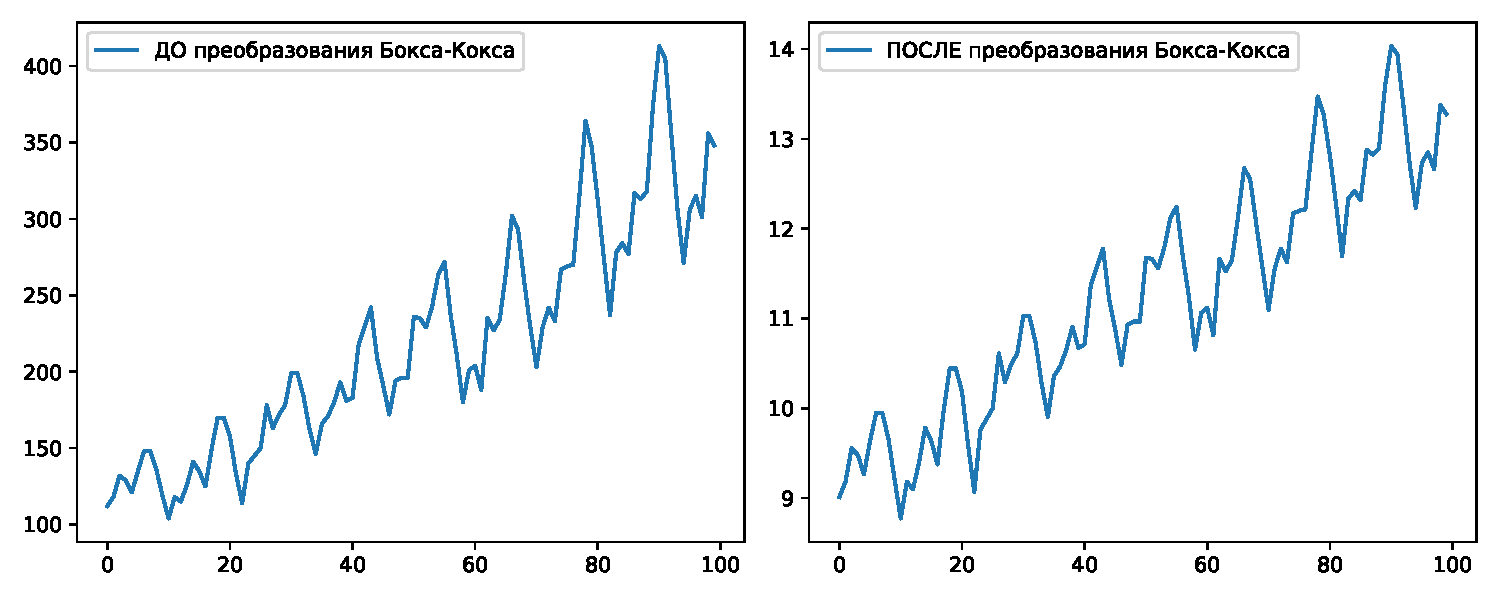
\includegraphics[scale=0.70]{figures/boxcox.pdf}
	\caption{Влияние преобразования Бокса-Кокса на временной ряд\\с изменяющейся во времени дисперсией}\label{fig:boxcox}
\end{figure}

Параметр $ \lambda $ можно подбирать так, чтобы дисперсия была как можно более стабильной во времени. Прямое и обратное преобразования Бокса-Кокса реализованы в библиотеках \texttt{scipy} и \texttt{statsmodels}
\begin{lstlisting}[
style = ironpython,
emph = {invboxcox},
numbers = none
]
from scipy.stats import boxcox
from statsmodels.tsa.hotwinters import (
                                        #boxcox,
                                        inv_boxcox
                                        )

# пользуемся готовым решением для обратного преобразования Бокса-Кокса
lmbda = 0.25
arr = np.array([3, 5, 10])
# можно задать значение ламбда самому или позволить вычислить его
arr_transformed = boxcox(arr, lmbda) # array([1.26429605, 1.98139512, 3.11311764])
arr_transformed, lmbda_compute = boxcox(arr)  # здесь lmbda вычисляется
                                              # с помощью максимизации логарифма правдоподобия
inv_boxcox(arr_transformed, lmbda)  # array([ 3.,  5., 10.])

# пишем свою реализацию обратного преобразования Бокса-Кокса
def invboxcox(arr: np.array, lmbda: np.float) -> np.array:
    if lmbda == 0:
        return (np.exp(arr))
    else:
        return (np.exp(np.log(lmbda*arr + 1)/lmbda))
\end{lstlisting}

Так как классическое преобразование Бокса-Кокса предполагает работу только с положительными величинами, то было предложено несколько модификаций, учитывающих нулевые и отрицательные значения. Самым очевидным вариантом является сдвиг всех значений на некоторую константу $ \alpha $ так, чтобы выполнялось условие $ (y_i + \alpha) > 0, \, i = 1,\dots, n $
\begin{align*}
	\hat{y}_i =
	\begin{cases}
		\log (y_i + \alpha), &\lambda = 0,\\
		\dfrac{(y_i + \alpha)^\lambda - 1}{\lambda}, &\lambda \neq 0.
	\end{cases}
\end{align*}




\section{Приемы работы с ETL-инструментом \texttt{Apache NiFi}}

<<Одиночный>> экземпляр \texttt{Apache NiFi} \url{https://nifi.apache.org/} можно создать с использованием Docker
\begin{lstlisting}[
style = bash,
numbers = none
]
docker run -d --name nifi -p 8080:8080 apache/nifi:latest
\end{lstlisting}

Экземпляр будет доступен через web-браузер по \verb|http://localhost:8080/nifi|.



\section{Приемы работы с пакетом \texttt{Vowpal Wabbit}}

\section{Приемы работы с библиотекой \texttt{BeautifulSoup}}

\subsection{Пример использования \texttt{BeautifulSoup} для скрапинга сайта}

В качестве простого примера извлечем имена руководителей компаний из группы компаний оборонного комплекса. Имена нужных тегов удобно искать с помощью специальных инструментов разработчика, доступных в веб-браузере. Например, в Yandex-браузере получить доступ к панели разработчика можно так \menu{Настройки > Дополнительно > Дополнительные инструменты > Инструменты разработчика}.
\begin{lstlisting}[
style = ironpython,
numbers = none
]
import requests
import pandas as pd
import psycopg2
from pprint import pprint
from bs4 import BeautifulSoup
from pandas import DataFrame, Series

main_url = 'http://ros-oborona.ru/koncerny.html'
res = requests.get(main_url)
soup = BeautifulSoup(res.text, features='lxml')

company_list = soup.find('div',
                         {'class' : 'elementor-text-editor elementor-clearfix'})
profile_list = company_list.find_all('td')

href_list = []
for elem in profile_list:
    try:
        href_list.append(elem.find('a').get('href'))
    except AttributeError:
        continue

heads_of_company_list = []
for company_url in href_list:
    res_elem = requests.get(company_url)
    soup_elem = BeautifulSoup(res_elem.text, features='lxml')
    head_of_company = soup_elem.find('span',
                                     {'class' : 'company-info__text'}).text
    if len(head_of_company.split()) == 3:
        heads_of_company_list.append(head_of_company.split())

heads_of_company_df = DataFrame(heads_of_company_list,
                                columns=['lastname', 'firstname', 'middlename'])
heads_of_company_df.index.name = 'id'
heads_of_company_df.to_csv('heads_of_company.csv', index=True)

# -- PostgreSQL
conn = psycopg2.connect('dbname=postgres user=postgres password=evdimonia')
cursor = conn.cursor()

heads_df = pd.read_csv('heads_of_company.csv')
heads_records = heads_df.to_dict('records')

cursor.execute(
            '''CREATE TABLE IF NOT EXISTS heads_of_company(
                   id integer primary key,
                   lastname text not null,
                   firstname text not null,
                   middlename text not null)'''
)
cursor.executemany(
            '''INSERT INTO heads_of_company(id, lastname, firstname, middlename)
                   VALUES (%(id)s, %(lastname)s, %(firstname)s, %(middlename)s)
                   ON CONFLICT DO NOTHING''', heads_records
)
conn.commit()

cursor.execute('SELECT * FROM heads_of_company')
fetchall = cursor.fetchall()
pprint(fetchall)
# выведет
# [(0, 'Мясников', 'Александр', 'Алексеевич'),
# (1, 'Медовщук', 'Ирина', 'Сергеевна'),
# (2, 'Матыцын', 'Александр', 'Петрович'),
# (3, 'Смирнова', 'Оксана', 'Константиновна'),
# ...]
\end{lstlisting}

\section{Приемы работы с библиотекой \texttt{pandas}}

\subsection{Число уникальных значений категориальных признаков в объекте \texttt{DataFrame}}

Для того чтобы вывести информацию по числу уникальных значений в каждом категориальном признаке некоторого объекта \texttt{pandas.DataFrame} можно воспользоваться конструкцией

\begin{lstlisting}[
style = ironpython,
numbers = none
]
X.select_dtypes('category').apply(lambda col: col.unique().shape[0])
\end{lstlisting}

\subsection{Число пропущенных значений в объекте \texttt{DataFrame}}

Информацию по числу пропущенных значений в каждом столбце можно вывести следующим образом

\begin{lstlisting}[
style = ironpython,
numbers = none
]
X.isna().any(axis=0)
\end{lstlisting}

\subsection{Управление стилями объекта \texttt{DataFrame}}

У объектов \texttt{DataFrame} есть стили и ими можно управлять, выделяя максимальные/минимальные значения в таблицы, значения, которые удовлетворяют какому-то специфическому условию и пр. Однако, эти приемы работают только в notebook'ах

\begin{lstlisting}[
style = ironpython,
numbers = none
]
import pandas as pd
import numpy as np
from pandas import DataFrame, Series

# определяем объект-DataFrame
m, n = 10, 4
df = DataFrame(np.random.randn(m, n),
               columns=[f'col{i}' for i in range(1, n+1)])
df.loc[[4, 6, 9], ['col1', 'col4']] = np.nan
\end{lstlisting}

\begin{lstlisting}[
style = ironpython,
emph = {threshold_color, background_color_max, backgournd_color_min},
numbers = none
]
from typing import List, TypeVar

# это способ обойти ограничения аннотаций для объектов pandas
ElemOfDataframe = TypeVar('DataFrame.iloc[int, int]')

# определяем функции для управления стилями объекта-DataFrame
def threshold_color(val: ElemOfDataframe) -> str:
    '''
    Значения большие 0.5, но меньшие 1.0 выделяет красным;
    Отрицательные значения выделяет синим;
    Все прочие значения печатаются черным
    '''
    return 'color : {}'.format('red' if ((val > 0.5) and (val < 1.0)) else
                               'blue' if val < 0. else 'black')

def background_color_max(col: Series) -> List[str]:
    '''
    Фон максимальных значений в столбце выделяется желтым.
    '''
    mask = col == col.max()  # булева маска
    return ['background-color : yellow' if bool_elem else '' for bool_elem in mask]

def background_color_min(col: Series) -> List[str]:
    '''
    Фон максимальных значений в столбце выделяется светло-зеленым.
    '''
    mask = col == col.min()  # булева маска
    return ['background-color : lightgreen' if bool_elem else '' for bool_elem in mask]
\end{lstlisting}

Работа со стилями объекта-DataFrame в ячейке выглядит следующим образом

\begin{lstlisting}[
style = ironpython,
numbers = none
]
(  # скобки здесь нужны для переноса строки без символа `\`
    df.style.
        applymap(threshold_color).
        apply(background_color_max).
        apply(background_color_min).
        format(
            {  # можно применять разные спецификаторы формата к разным столбцам
                'col2' : '{:.5e}',
                'col4' : '{:.3G}'
            }
        )
)
\end{lstlisting}

Результат будет выглядеть как на \pic{fig:format-df}.

\begin{figure}[h]
	\centering
	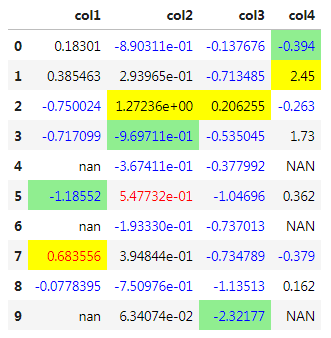
\includegraphics[scale=1]{figures/format_df.png}
	\caption{ Отформатированный вывод \texttt{DataFrame} }\label{fig:format-df}
\end{figure}

Еще одно очень полезное применение этого приема: можно раскрашивать наиболее частые значения категориального признака

\begin{lstlisting}[
style = ironpython,
emph = {color_code_freq_cat},
numbers = none
]
from typing import List

def color_code_freq_cat(col: Series) -> List[str]:
    '''
    Раскрашивает самые частые значения категориальных столбцов
    '''
    # принимает столбец-Series `col`
    freq_cat = col.value_counts().index[0]  # самое частое значение категории
    return ['color : {}'.format('red' if elem == freq_cat else 'black') for elem in col]

df = DataFrame({'col1' : list('abbbabbaaab'),
                'col2' : list('cdcccddcscd'),
                'col3' : np.random.randn(11)})

# apply работает со столбцами или строками
df_test.iloc[:5].select_dtypes('object').style.apply(color_code_freq_cat)
\end{lstlisting}

Результат приведен на \pic{fig:color-code-freq-cat}. Вывести самое частое значение в каждом столбце можно с помощью конструкции

\begin{lstlisting}[
style = ironpython,
numbers = none
]
# apply работает со столбцами или строками
df.apply(lambda col: col.value_counts().index[0])
\end{lstlisting}

\begin{figure}[h]
	\centering
	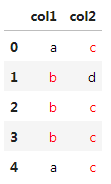
\includegraphics[scale=1]{figures/color_code_freq_cat.png}
	\caption{ Результат применения функции \texttt{color\_code\_freq\_cat} }\label{fig:color-code-freq-cat}
\end{figure}


\section{Приемы работы с библиотекой \texttt{Plotly}}

Рассмотрим простой пример работы с библиотекой \texttt{plotly} в блокноте
\begin{lstlisting}[
style = ironpython,
numbers = none
]
import numpy as np
import chart_studio.plotly as py
import plotly.graph_objs as go
from plotly.offline import (
    download_plotlyjs,
    init_notebook_mode,
    plot,
    iplot
)
init_notebook_mode(connected=True)

# в текущей директории будет создан html-файл, а график откроется в браузере
plot(go.Figure(data=[
    go.Scatter(y=np.random.randn(100).cumsum()),
    go.Scatter(y=np.random.randn(100).cumsum())
]), filename='file_name.html')
\end{lstlisting}




\section{Интерпретация моделей и оценка важности признаков с библиотекой \texttt{SHAP}}

\subsection{Общие сведения о значениях Шепли}

В библиотеке \texttt{SHAP} \url{https://github.com/slundberg/shap} для оценки \emph{важности признаков} используются \emph{значения Шепли}\footnote{Термин пришел из теории кооперативных игр} (Shapley value) \url{https://en.wikipedia.org/wiki/Shapley_value}.

Или несколько точнее: при построении \emph{локальной} интерпретации (то есть интерпретации на конкретной точке данных) значения Шепли, строго говоря, оценивают \emph{силу влияния}\footnote{Еще эту оценку можно интерпретировать как \emph{вклад}} $ i $-ого признака $ f_i $ на значения целевого вектора $ y $, а вот \emph{важность признака} в контексте модели можно оценить при построении \emph{глобальной} интерпретации с помощью значений Шепли, взятых по абсолютной величине и усредненных по имеющемуся набору данных. 

\remark{
Значения Шепли объясняют как <<справедливо>> оценить вклад каждого признака в прогноз модели
}

Значения Шепли $i$-ого признака на \emph{конкретном объекте} (на текущей точке данных) вычисляются следующим образом (здесь сумма распространяется на все подмножества признаков $ S $ из множества признаков $ N $, не содержащие $ i $-ого признака)
\begin{align*}
\phi_i(v) = \sum_{S \subseteq N\setminus\{i\}} \dfrac{|S|!(n - |S| - 1)!}{n!}\Bigl( \underset{f_i-contribution }{\underbrace{ v(S \cup \{i\}) - v(S)}} \Bigr),
\end{align*}
где $ n $ -- общее число признаков; $ v(S \cup \{i\}) $ -- прогноз модели с учетом $ i $-ого признака; $ v(S) $ -- прогноз модели без $ i $-ого признака.

Выражение $ v(S \cup \{i\}) - v(S) $ -- это вклад $ i $-ого признака. Если теперь вычислить среднее вкладов по всем возможным перестановкам, то получится <<честная>> оценка вклада $ i $-ого признака.

Значение Шепли для $ i $-ого признака вычисляется для каждой точки данных (например, для каждого клиента в выборке) на всех возможных комбинациях признаков (в том числе и для пустых подмножеств $ S $).

\remark{
Метод анализа важности признаков, реализованный в библиотеке \texttt{SHAP}, является и \emph{согласованным}, и \emph{точным} (см. \href{https://towardsdatascience.com/interpretable-machine-learning-with-xgboost-9ec80d148d27}{Interpretable Machine Learning with XGBoost})
}



\subsection{ Пример построения локальной и глобальной интерпретаций }

Примеры использования библиотеки \texttt{SHAP} не только для tree-base моделей можно найти по адресу \url{https://github.com/slundberg/shap/tree/master/notebooks/tree_explainer}.

Решается задача регрессии для классического набора данных \texttt{boston}. Требуется предсказать стоимость квартиры. 

\begin{lstlisting}[
style = ironpython,
numbers = none
]
import shap
import os
import pandas as pd
import numpy as np
from pandas import DataFrame, Series
import matplotlib.pyplot as plt
from sklearn.ensemble import RandomForestRegressor, GradientBoostingRegressor
from sklearn.model_selection import train_test_split
from sklearn.datasets import load_boston
#%matplotlib inline  # если код оформляется в JupyterLab
#shap.initjs()  # если код оформляется в JupyterLab

boston = load_boston()
X, y = boston['data'], boston['target']  # numpy-массивы

# объекты pandas
X_full = DataFrame(X, columns=boston['feature_names'])
y_full = Series(y, name = 'PRICE')

X_train, X_test, y_train, y_test = train_test_split(X_full, y_full, random_state=42)

rf = RandomForestRegressor(n_estimators=500).fit(X_train, y_train)

explainer = shap.TreeExplainer(rf)  # <- NB
shap_values_train = explainer.shap_values(X_train)  # <- NB
\end{lstlisting}

\subsubsection{Локальная интерпретация отдельной точки данных обучающего набора}

Теперь можно построить локальную интерпретацию для одной точки данных из обучающего набора (см. \pic{fig:shap_force_plt_train})

\begin{lstlisting}[
style = ironpython,
title = {\sffamily К вопросу о локальной интерпретации отдельной точки данных обучающего набора},
numbers = none
]
row = 1
shap.force_plot(
    explainer.expected_value,  # ожидаемое значение
    shap_values_train[row, :],  # 2-ая строка в матрице значений Шепли
    X_train.iloc[row, :]  # 2-ая строка в обучающем наборе данных
)
\end{lstlisting}

Можно считать, что \texttt{explainer.expected\_value} это значение, полученное усреднением целевого вектора по точкам обучающего набора данных, т.е. \texttt{y\_train.mean()}.

\begin{figure}[h]
	\centering
	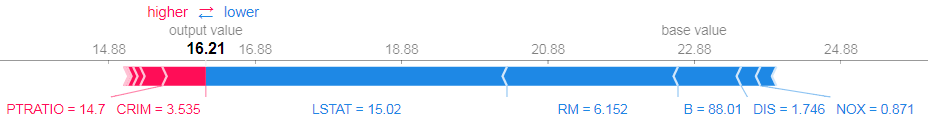
\includegraphics[scale=0.80]{figures/shap_force_plt_train.png}
	\caption{ Локальная интерпретация для одной точки данных обучающего набора }\label{fig:shap_force_plt_train}
\end{figure}

Еще можно построить график частичной зависимости (\pic{fig:shap_dependence_plt_train})

\begin{lstlisting}[
style = ironpython,
numbers = none
]
shap.dependence_plot('LSTAT', shap_values, X_train)
\end{lstlisting}

\begin{figure}[h]
	\centering
	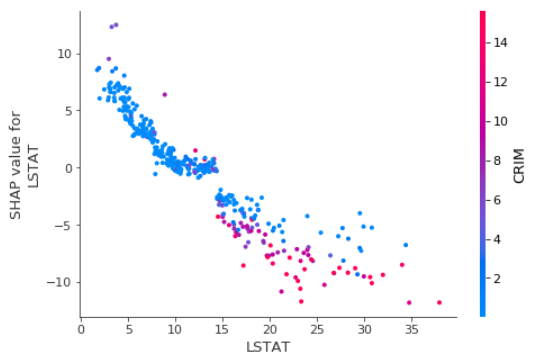
\includegraphics[scale=0.85]{figures/shap_dependence_plt_train.png}
	\caption{ График частичной зависимости признака \texttt{LSTAT} от значений Шепли\\с учетом влияния признака \texttt{CRIM} }\label{fig:shap_dependence_plt_train}
\end{figure}

\subsubsection{Локальная интерпретация отдельной точки данных тестового набора}

Прежде чем приступить к вычислению значений Шепли, следует создать поверхностную копию тестового набора данных

\begin{lstlisting}[
style = ironpython,
numbers = none
]
X_test_for_pred = X_test.copy()
X_test_for_pred['predict'] = np.round(rf.predict(X_test), 2)

explainer = shap.TreeExplainer(rf)
# вычисляем значения Шепли для тестового набора данных со столбцом 'predict'
shap_values_test = explainer.shap_values(X_test_for_pred)
\end{lstlisting}

Теперь можно построить локальную интерпретацию для отдельной точки данных тестового набора (\pic{fig:shap_dependence_plt_test}).

\begin{figure}
	\centering
	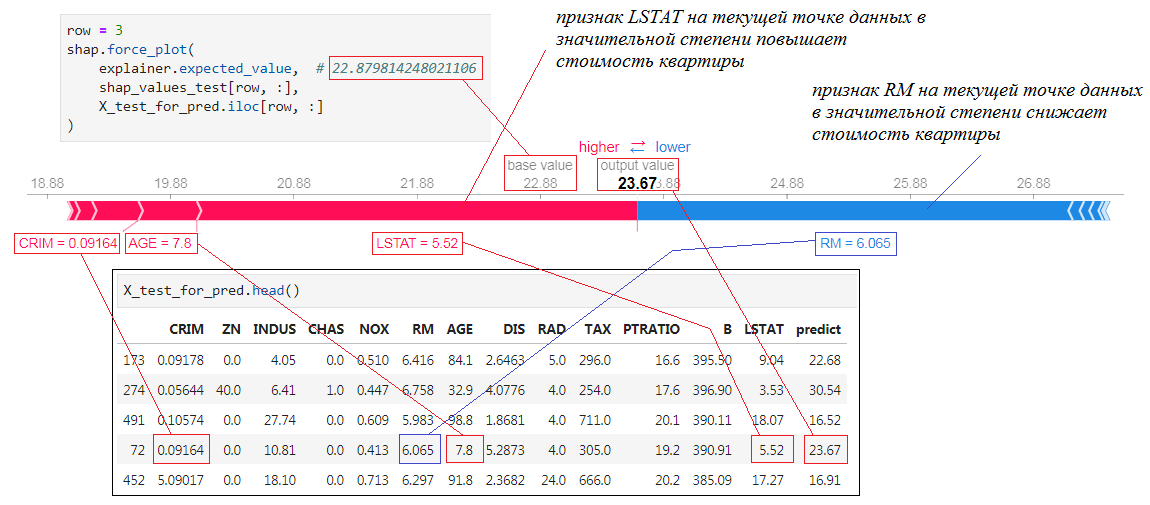
\includegraphics[scale=0.7]{figures/shap_dependence_plt_test.png}
	\caption{ Локальная интерпретация для одной точки данных тестового набора }\label{fig:shap_dependence_plt_test}
\end{figure}

Из \pic{fig:shap_dependence_plt_test} видно, что признаки с различной <<силой>>\footnote{Ширина полосы}, которая определяется значениями Шепли, смещают предсказание модели на данной точке. Например, признак \texttt{LSTAT} (процент населения с низким социальным статусом) в значительной степени \emph{повышает}\footnote{Потому что значение этого признака невелико; чем меньше процент населения с низким социальным статусом проживает в округе, тем выше стоимость квартиры} стоимость квартиры на \underline{данной точке} по отношению к базовому значению \texttt{base\_value}, а признак \texttt{RM} (среднее число комнат в жилом помещении) в значительной степени снижает.

\begin{lstlisting}[
style = ironpython,
title = {\sffamily К вопросу о локальной интерпретации отдельной точки данных тестового набора},
numbers = none
]
row = 3
shap.force_plot(
    explainer.expected_value,  # 22.879814248021106
    #y_train.mean()  # 22.907915567282323
    shap_values_test[row, :],
    X_test_for_pred.iloc[row, :]
)
\end{lstlisting}

\subsubsection{Глобальная интерпретация модели на тестовом наборе данных}

Удобно работать с диаграммой рассеяния \texttt{shap.summary\_plot} (\pic{fig:summary_plt_test}), на которой изображаются признаки в порядке убывания их важности, с одновременным указанием того, насколько сильно каждый из признаков влияет на целевую переменную.

\begin{lstlisting}[
style = ironpython,
numbers = none
]
shap.summary_plot(shap_values_test, X_test_for_pred)
\end{lstlisting}

\begin{figure}[h]
	\centering
	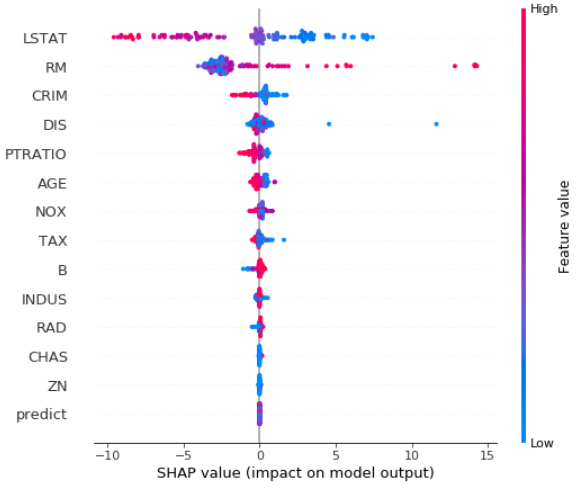
\includegraphics[scale=0.85]{figures/summary_plt_test.png}
	\caption{ Диаграмма рассеяния для точек тестового набора данных }\label{fig:summary_plt_test}
\end{figure}

Какие выводы можно сделать из \pic{fig:summary_plt_test}:

\begin{itemize}
	\item Признаки \texttt{LSTAT}, \texttt{RM} и \texttt{CRIM} имеют высокую важность для модели в целом,
	
	\item Для признака \texttt{LSTAT} наблюдается отрицательная статистическая зависимость от целевой переменной, т.е. низкие значения этого признака отвечают высоким значениям целевой переменной (стоимости на квартиру),
	
	\item Для признака \texttt{RM} наблюдается положительная статистическая зависимость от целевой переменной: чем больше комнат в жилом помещении, тем выше стоимость квартиры.
\end{itemize}

Затем можно детальнее изучить графики частичной зависимости, построенные на тестовом наборе данных. Рассмотрим зависимость признака \texttt{CRIM} (уровень преступности в городе на душу населения) от значений Шепли, вычисленных для этого признака (\pic{fig:dependeces_plt_test_CRIM}).

\begin{lstlisting}[
style = ironpython,
numbers = none
]
shap.dependence_plot('CRIM', shap_values_test[:, :-1], X_test_pred.iloc[:, :-1])
\end{lstlisting}

\begin{figure}[h!]
	\centering
	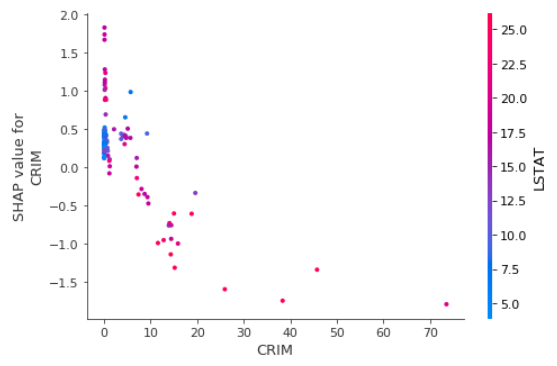
\includegraphics[scale=0.85]{figures/dependeces_plt_test_CRIM.png}
	\caption{ График частичной зависимости признака \texttt{CRIM} от значений Шепли\\с учетом влияния \texttt{LSTAT} }\label{fig:dependeces_plt_test_CRIM}
\end{figure}

Какие выводы можно сделать из \pic{fig:dependeces_plt_test_CRIM}:

\begin{itemize}
	\item Чем выше уровень преступности в городе, тем в большей степени снижается стоимость квартиры,
	
	\item Не везде, где проживает высокий процент населения с низким социальным статусом наблюдается высокий уровень преступности, однако в тех местах, где регистрируется высокий уровень преступности одновременно регистрируется и высокий процент населения с низким социальным статусом.
\end{itemize}


\section{Перестановочная важность признаков в библиотеке \texttt{eli5}}


Еще важность признаков можно оценивать с помощью так называемой \emph{перестановочной важности} (permutation importances) \url{https://www.kaggle.com/dansbecker/permutation-importance}.

Идея проста: нужно в заранее отведенном для исследования важности признаков наборе данных (валидационном наборе) перетасовать значения признака, влияние которого изучается на данной итерации, оставив остальные признаки (столбцы) и целевой вектор без изменения.

Признак считается <<важным>>, если метрики качества модели падают, и соответственно -- <<неважным>>, если перестановка не влияет на значения метрик. Перестановочная важность вычисляется после того как модель будет обучена.

\remark{
Перестановочная важность обладает свойством \emph{согласованности}, но не обладает свойством \emph{точности} \href{https://towardsdatascience.com/interpretable-machine-learning-with-xgboost-9ec80d148d27}{Interpretable Machine Learning with XGBoost}
}

Рассмотрим задачу построения регрессионной модели на наборе данных \texttt{load\_boston}

\begin{lstlisting}[
style = ironpython,
numbers = none
]
import eli5
import pandas as pd
from eli5.sklearn import PermutationImportance
from sklearn.ensemble import RandomForestRegressor
from sklearn.model_selection import train_test_split
from sklearn.datasets import load_boston
from pandas import DataFrame, Series

boston = load_boston()

X_train, X_test, y_train, y_test = train_test_split(boston['data'],
                                                    boston['target'], 
                                                    random_state=2)

X_train_sub, X_valid, y_train_sub, y_valid = train_test_split(X_train,
                                                              y_train,
                                                              random_state=0)

# модель случайного леса, как обычно, обучается на обучающей выборке
rf = RandomForestRegressor(n_estimators=500).fit(X_train_sub, y_train_sub)

# модель перестановочной важности обучается на валидационном наборе данных
perm = PermutationImportance(rf, random_state=42).fit(X_valid, y_valid)

eli5.show_weights(perm, feature_names = boston['feature_names'])  # визуализирует перестановочные важности признаков
\end{lstlisting}

\section{Регулярные выражения в \texttt{Python}}

В языке \texttt{Python} есть несколько тонких особенностей, связанных с регулярными выражениями, а имеено с поведением жадных и нежадных квантификаторов. Рассмотрим пример с \emph{жадным} квантификатором
\begin{lstlisting}[
style = ironpython,
numbers = none
]
# python
import re
re.compile('y*(\d{1,3})').search('xy1234z').groups()[0]  # '123'
\end{lstlisting}

Аналогичный результат получается и в \texttt{PostgreSQL}
\begin{lstlisting}[
style = sql,
numbers = none
]
-- postgresql
select substring('xy1234z', 'y*(\d{1,3})'); -- '123'
\end{lstlisting}

Но если используется \emph{нежадный} квантификатор, то результаты будут различаться
\begin{lstlisting}[
style = ironpython,
numbers = none
]
# python
import re
re.compile('y*?(\d{1,3})').search('xy1234z').groups()[0]  # '123'
\end{lstlisting}

А вот в \texttt{PostgreSQL}
\begin{lstlisting}[
style = sql,
numbers = none
]
-- postgresql
select substring('xy1234z', 'y*?(\d{1,3})'); -- '1'
\end{lstlisting}

Совпадать результаты будут только в том случае, если в регулярном выражении \texttt{Python} специально указать, что \verb|{m,n}| должен быть нежадным, т.е. \verb|{m,n}?|
\begin{lstlisting}[
style = ironpython,
numbers = none
]
# python
import re
re.compile('y*?(\d{1,3}?)').search('xy1234z').groups()[0]  # '1'
\end{lstlisting}


\listoffigures\addcontentsline{toc}{section}{Список иллюстраций}

% Источники в "Газовой промышленности" нумеруются по мере упоминания 
\begin{thebibliography}{99}\addcontentsline{toc}{section}{Список литературы}
	\bibitem{lutz:learningpython-2011}{{\emph{Лутц М.} Изучаем Python, 4-е издание. -- Пер. с англ. -- СПб.: Символ-Плюс, 2011. -- 1280~с. }
		
	\bibitem{beazley:python-2010}{\emph{Бизли Д.} Python. Подробный справочник. -- Пер. с англ. -- СПб.: Символ-Плюс, 2010. -- 864~с. }
	
	\bibitem{chacon:2020}{ \emph{Чакон С.}, \emph{Штрауб Б.} Git для профессионального программиста. -- СПб.: Питер, 2020. -- 496~с. }
	
	\bibitem{ramalho:python-2016}{\emph{Рамальо Л.}{ Python. К вершинам мастерства. -- М.: ДМК Пресс, 2016. -- 768 с.}}
	
	\bibitem{slatkin:python-2016}{ \emph{Слаткин  Б.} Секреты Python: 59 рекомендаций по написанию эффективного кода. -- М.: ООО~<<И.Д. Вильямс>>, 2016. -- 272~с.}
	
	\bibitem{prohorenok:python-2016}{ \emph{Прохоренок Н.А.}, \emph{Дронов В.А.} Python 3 и PyQt 5. Разработка приложений. -- СПб.: БХВ-Петербург, 2016. -- 832~с.}
	
	\bibitem{chandola:2009}{\emph{Chandola V.}, \emph{Banerjee A.} etc. } Anomaly detection: A survey, ACM Computing Surveys, vol. 41(3), 2009, pp. 1--58.
\end{thebibliography}

\end{document}